\documentclass[12pt,a4paper]{article}
\usepackage[utf8]{inputenc}
\usepackage{amsmath}
\usepackage{amsfonts}
\usepackage{amssymb}
\usepackage{graphicx}
\usepackage[hidelinks]{hyperref}
\usepackage{booktabs}
\usepackage{longtable}
\usepackage{geometry}
\usepackage{fancyhdr}
\usepackage{caption}
\usepackage{subcaption}
\usepackage{listings}
\usepackage{xcolor}
\usepackage{float}
\usepackage{array}
\usepackage{multirow}
\usepackage{tikz}
\usetikzlibrary{shapes.geometric, arrows, positioning, fit}

\geometry{margin=1in}
\setlength{\headheight}{14.5pt}
\pagestyle{fancy}
\fancyhf{}
\rhead{Bonita BPM Projects}
\lhead{Business Intelligence}
\rfoot{\thepage}

% Define colors for code listings
\definecolor{codegreen}{rgb}{0,0.6,0}
\definecolor{codegray}{rgb}{0.5,0.5,0.5}
\definecolor{codepurple}{rgb}{0.58,0,0.82}
\definecolor{backcolour}{rgb}{0.95,0.95,0.92}

% Hyperref setup
\hypersetup{
    colorlinks=true,
    linkcolor=blue,
    filecolor=magenta,
    urlcolor=cyan,
    pdftitle={Bonita BPM Business Process Management},
    pdfpagemode=FullScreen,
}

% Code listing style
\lstdefinestyle{mystyle}{
    backgroundcolor=\color{backcolour},
    commentstyle=\color{codegreen},
    keywordstyle=\color{magenta},
    numberstyle=\tiny\color{codegray},
    stringstyle=\color{codepurple},
    basicstyle=\ttfamily\footnotesize,
    breakatwhitespace=false,
    breaklines=true,
    captionpos=b,
    keepspaces=true,
    numbers=left,
    numbersep=5pt,
    showspaces=false,
    showstringspaces=false,
    showtabs=false,
    tabsize=2
}

\lstset{style=mystyle}

\begin{document}

\begin{titlepage}
\centering
\textbf{Universit\`a degli Studi di Napoli Federico II}\\
\textbf{Data Science}\\[10mm]

Business Intelligence \break

\begin{figure}[h!]
\begin{center} 
\includegraphics[height=8cm]{figures/uni-logo.png}
\end{center}
\end{figure}

\textbf{Zain Abbas} \\[2mm]
\textbf{Airaf Siddiqui} \\[2mm]
\textbf{Adil Shahzad} \\[2cm]

\textbf{Business Process Management with Bonita: DEUCE Credit Recovery and IDEA Labor Disputes} \\[5mm]

Project Report\\[1cm]

\textbf{FLORA AMATO}\\
\null\vfill

Naples, \the\year

\end{titlepage}

\newpage

\tableofcontents

\newpage

\listoffigures
\listoftables

\newpage

\begin{abstract}
This report presents the design and implementation of two business processes using Bonita BPM (Business Process Management) software, developed as part of the Business Intelligence course project. The work addresses two European Union digitization initiatives: \textbf{DEUCE} (Digital Uncontested European Credit Enforcement) for cross-border monetary credit recovery, and \textbf{IDEA} (Intelligent Digitization for European Access to justice) for labor dispute procedure selection. Contest 2 implements a three-lane workflow (Citizen, Clerk, Judge) with 3 human tasks, 2 XOR gateways, and 19 Business Data Model attributes for processing credit applications. Contest 3 implements a two-lane workflow (Worker, Office) with 4 human tasks, 1 XOR gateway, and 30 BDM attributes, featuring a novel dual-tracking system for worker preferences versus office confirmations. Both processes utilize Bonita's Business Data Model for form integration and data persistence, with gateway conditions implemented in Groovy expressions. The implementations demonstrate proper BPMN notation, actor-based access control, and comprehensive form design patterns suitable for judicial digitization workflows.

\textbf{Keywords:} Business Process Management, BPMN, Bonita BPM, Workflow Automation, EU Digitization, Credit Recovery, Labor Disputes, Business Data Model
\end{abstract}

\newpage

\section{Introduction}

\subsection{Background and Motivation}

Business Process Management (BPM) represents a systematic approach to improving an organization's workflows through the design, modeling, execution, monitoring, and optimization of business processes. In the context of European Union judicial systems, BPM technologies offer significant potential for digitizing traditionally paper-based procedures, improving accessibility, and reducing processing times.

The European Commission has launched several initiatives to digitize justice systems across member states, addressing challenges such as:

\begin{enumerate}
    \item \textbf{Cross-Border Complexity}: Legal procedures spanning multiple jurisdictions require interoperable digital workflows
    \item \textbf{Manual Processing}: Traditional paper-based systems create delays and reduce traceability
    \item \textbf{Access to Justice}: Digital platforms can improve citizen access to legal procedures
    \item \textbf{Standardization}: Common digital frameworks enable consistent processing across courts
\end{enumerate}

This project implements two such digitization initiatives using Bonita BPM: the DEUCE project for credit recovery and the IDEA project for labor dispute resolution.

\subsection{Project Scope and Objectives}

This project develops two complete business processes in Bonita BPM:

\begin{itemize}
    \item \textbf{Contest 2 - DEUCE}: A monetary credit recovery workflow with three actors (Citizen, Clerk, Judge) and binary decision points for application completeness and legal approval
    \item \textbf{Contest 3 - IDEA}: A labor dispute procedure selection workflow with two actors (Worker, Office) featuring preference tracking and case preparation branches
\end{itemize}

The primary objectives are:
\begin{enumerate}
    \item Design BPMN-compliant process diagrams with proper swimlane architecture
    \item Implement Business Data Models (BDM) for structured data management
    \item Create user forms with appropriate read-only and editable sections
    \item Configure XOR gateways with Groovy-based routing conditions
    \item Validate processes through multiple test scenarios
\end{enumerate}

\subsection{Contributions}

This work makes the following contributions:
\begin{enumerate}
    \item \textbf{Complete BPM Implementation}: Two fully functional Bonita processes with forms, BDM, and gateway logic
    \item \textbf{EU Legal Framework Alignment}: Processes designed according to DEUCE and IDEA project requirements
    \item \textbf{Dual-Tracking System}: Novel implementation of preference vs. confirmation tracking in Contest 3
    \item \textbf{Comprehensive Documentation}: Detailed specifications for BDM attributes, form fields, and gateway conditions
    \item \textbf{Reproducible Methodology}: Step-by-step guidance for process recreation and testing
\end{enumerate}

\section{Bonita BPM Platform}

\subsection{Platform Overview}

Bonita BPM (Community Edition) is an open-source business process management platform that provides tools for process modeling, form design, and workflow execution. The platform consists of two primary components:

\begin{itemize}
    \item \textbf{Bonita Studio}: Development environment for designing BPMN diagrams, Business Data Models, and user forms
    \item \textbf{Bonita Portal}: Runtime environment for executing processes, managing tasks, and monitoring workflow progress
\end{itemize}

\subsection{Architecture}

\begin{figure}[H]
\centering
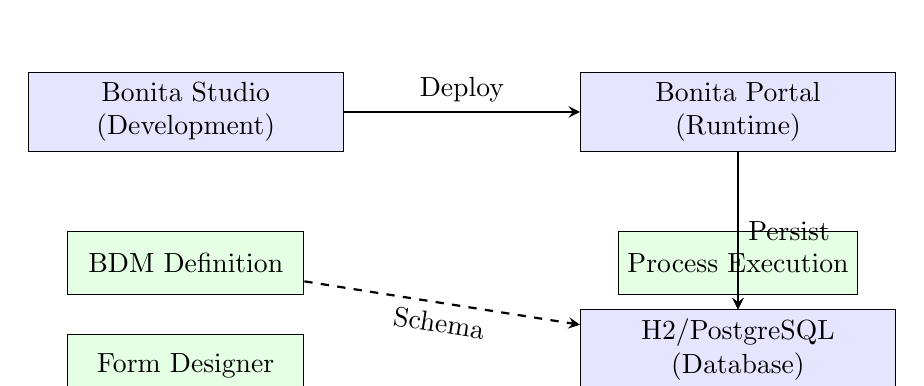
\begin{tikzpicture}[
    node distance=1.5cm,
    box/.style={rectangle, draw, minimum width=4cm, minimum height=1cm, align=center, fill=blue!10},
    smallbox/.style={rectangle, draw, minimum width=3cm, minimum height=0.8cm, align=center, fill=green!10},
    arrow/.style={->, >=stealth, thick}
]
    % Main components
    \node[box] (studio) {Bonita Studio\\(Development)};
    \node[box, right=3cm of studio] (portal) {Bonita Portal\\(Runtime)};
    \node[box, below=2cm of portal] (db) {H2/PostgreSQL\\(Database)};

    % Sub-components
    \node[smallbox, below=1cm of studio] (bdm) {BDM Definition};
    \node[smallbox, below=0.5cm of bdm] (forms) {Form Designer};
    \node[smallbox, below=1cm of portal] (exec) {Process Execution};

    % Arrows
    \draw[arrow] (studio) -- (portal) node[midway, above] {Deploy};
    \draw[arrow] (portal) -- (db) node[midway, right] {Persist};
    \draw[arrow, dashed] (bdm) -- (db) node[midway, below, sloped] {Schema};
    \draw[arrow, dashed] (exec) -- (db);
\end{tikzpicture}
\caption{Bonita BPM Architecture: Development to Execution Flow}
\label{fig:architecture}
\end{figure}

\begin{figure}[H]
\centering
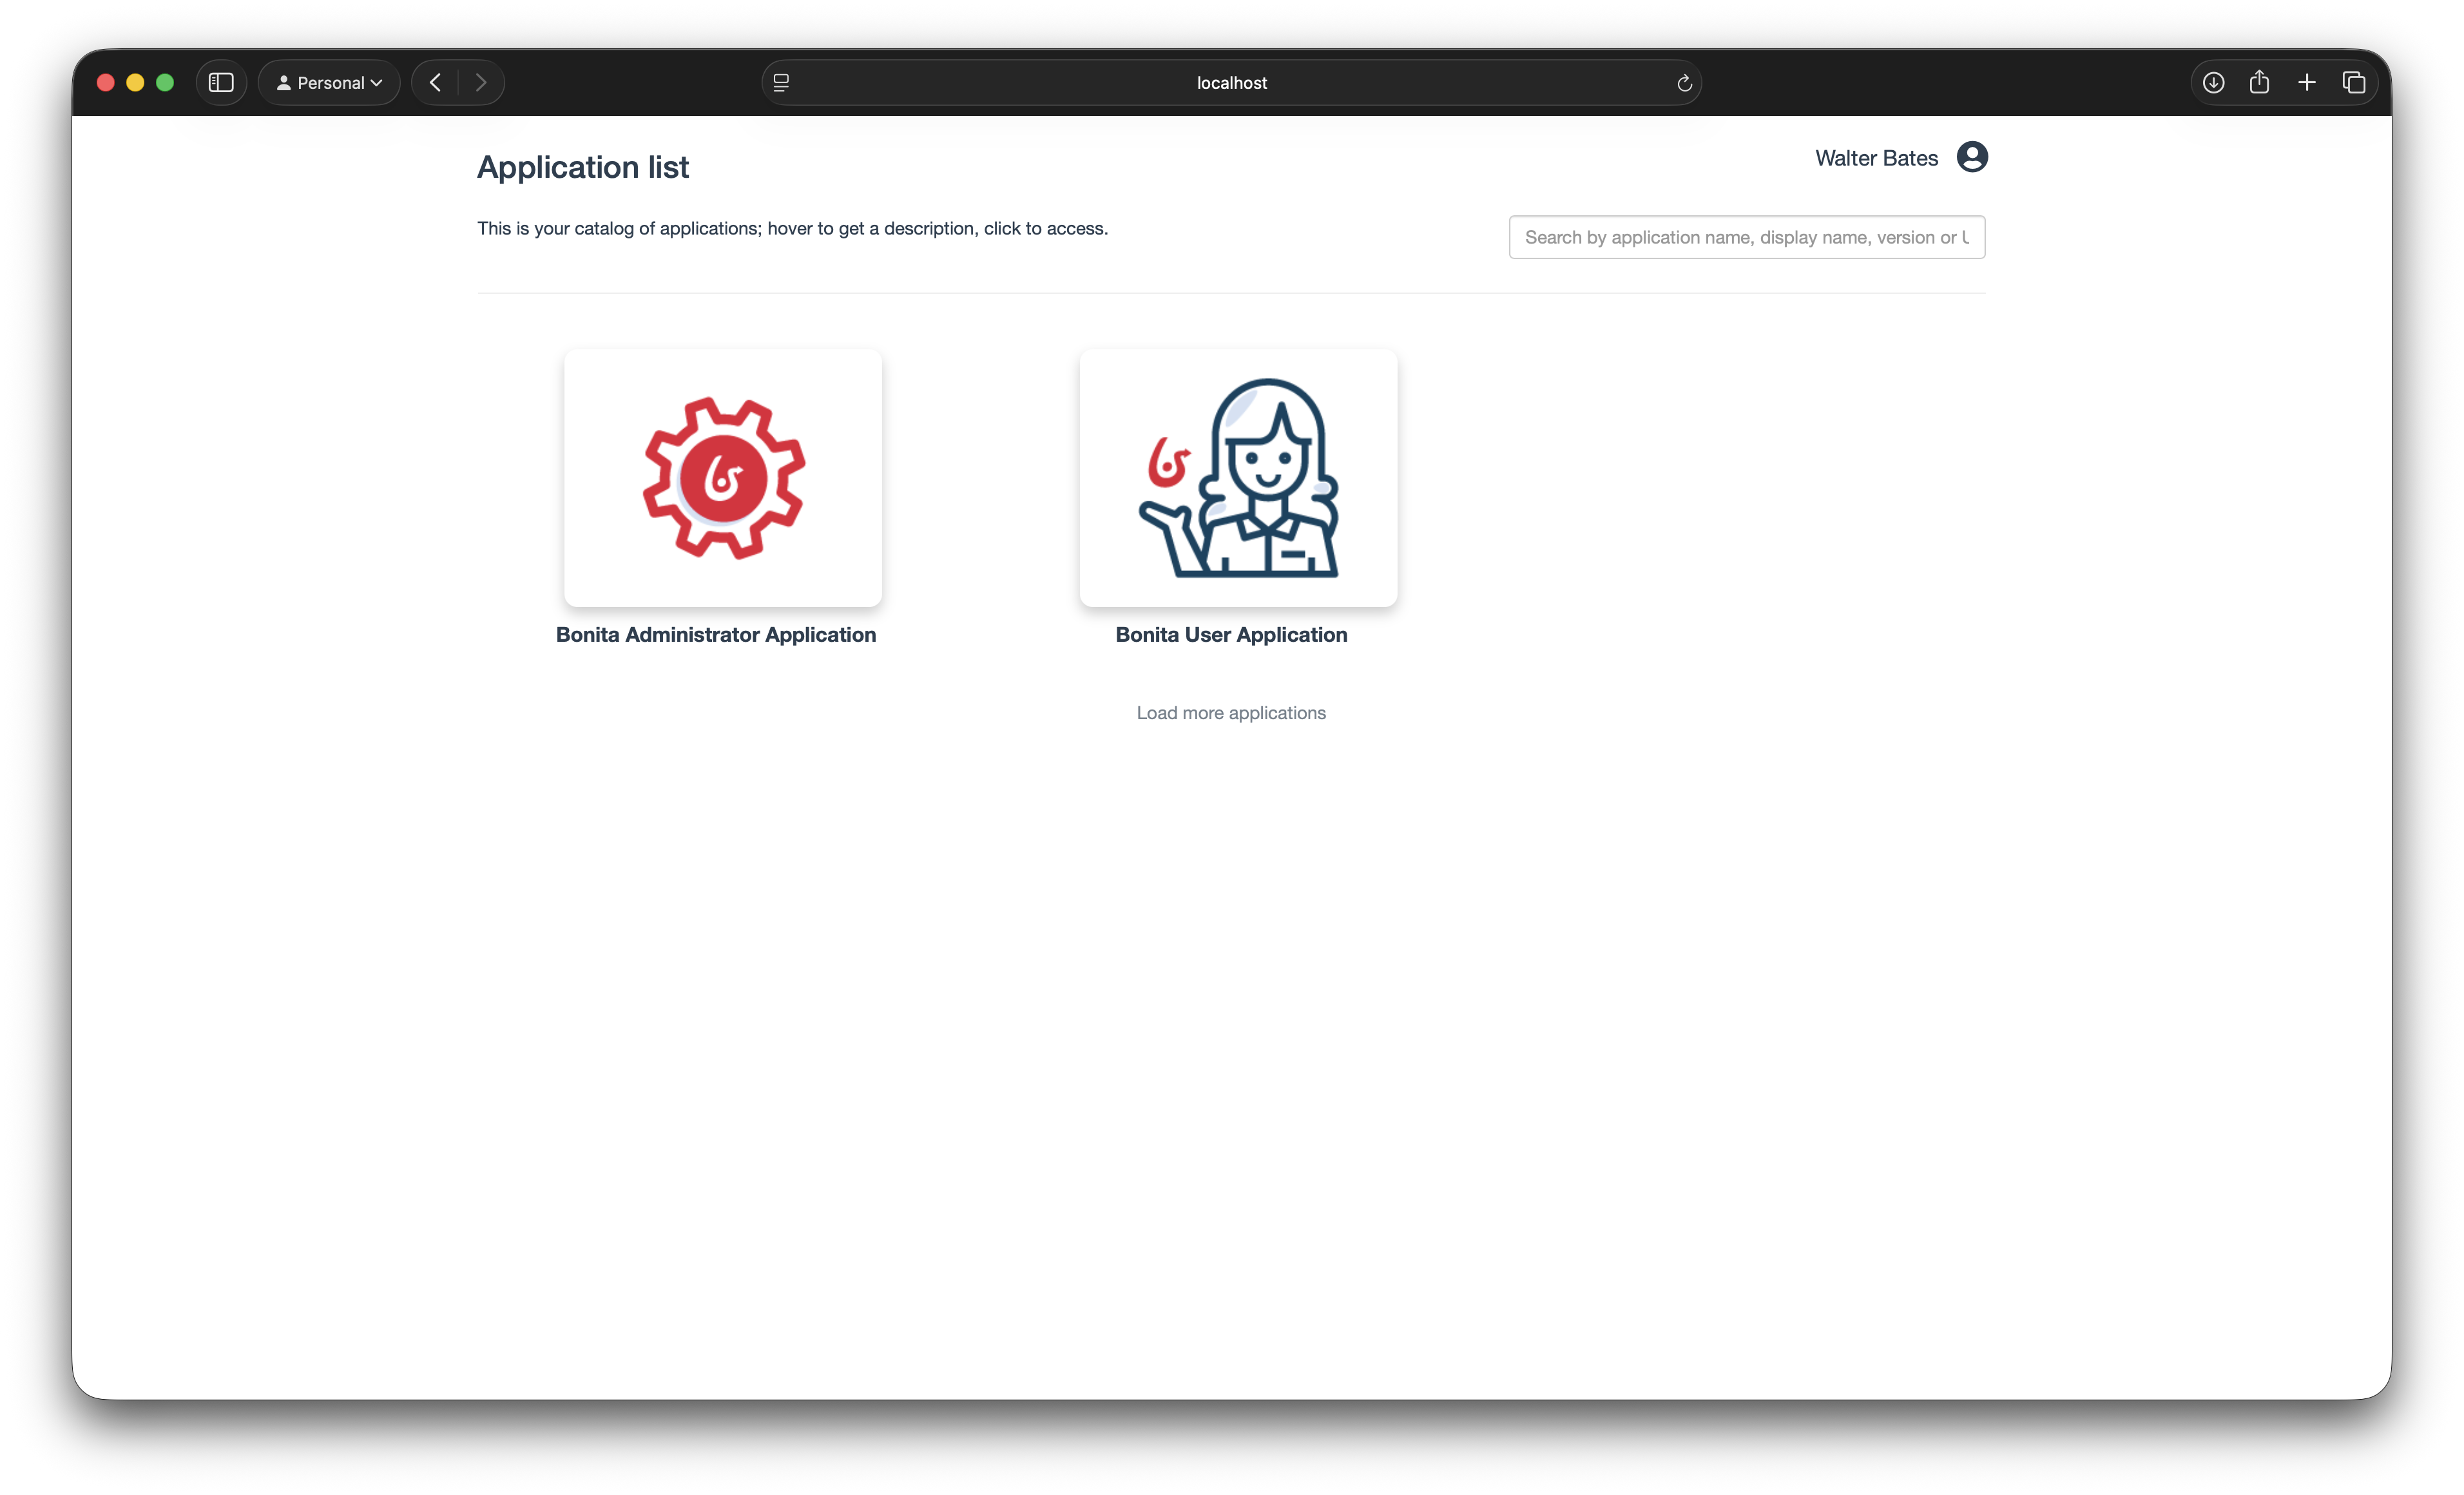
\includegraphics[width=0.9\textwidth]{figures/bonita_portal.png}
\caption{Bonita Portal Interface: Task management and process monitoring environment where users execute workflow tasks and administrators monitor process instances.}
\label{fig:portal}
\end{figure}

\subsection{Key Concepts}

\begin{table}[H]
\centering
\caption{Bonita BPM Key Concepts}
\begin{tabular}{lp{9cm}}
\toprule
\textbf{Concept} & \textbf{Description} \\
\midrule
Pool & Container for a complete process, representing a single workflow \\
Lane (Swimlane) & Horizontal subdivision within a pool, representing an actor or role \\
Human Task & Activity requiring user interaction through a form \\
XOR Gateway & Exclusive decision point routing flow based on conditions \\
Business Data Model & Structured data objects persisted in the database \\
Business Variable & Process-scoped instance of a BDM object \\
Form & User interface for task completion with data bindings \\
Actor Mapping & Configuration linking lanes to user groups/roles \\
\bottomrule
\end{tabular}
\label{tab:concepts}
\end{table}

\subsection{Business Data Model vs Process Variables}

A critical implementation decision involves choosing between Process Variables and Business Data Model (BDM) for data management:

\begin{table}[H]
\centering
\caption{BDM vs Process Variables Comparison}
\begin{tabular}{lcc}
\toprule
\textbf{Aspect} & \textbf{Process Variables} & \textbf{BDM} \\
\midrule
Form Integration & Manual contract setup & ``Add from data...'' works \\
Data Persistence & Process instance only & Database storage \\
Reusability & Single process & Across processes \\
Complex Types & Limited & Full object support \\
\textbf{Recommended} & No & \textbf{Yes} \\
\bottomrule
\end{tabular}
\label{tab:bdm_comparison}
\end{table}

Both Contest 2 and Contest 3 implementations use Business Variables from the BDM, enabling seamless form widget binding and persistent data storage.

\section{Contest 2: DEUCE Credit Recovery}

\subsection{Business Context}

DEUCE (Digital Uncontested European Credit Enforcement) is a European project focused on digitizing procedures for recovering uncontested monetary claims within the EU. The project addresses:

\begin{itemize}
    \item \textbf{European Payment Order (EPO)}: Simplified procedure for cross-border debt recovery
    \item \textbf{European Enforcement Order (EEO)}: Mechanism for enforcing judgments across member states
    \item \textbf{e-CODEX Infrastructure}: Technical framework for judicial system interoperability
\end{itemize}

The implemented workflow represents a basic credit recovery case where a citizen submits an application, a clerk verifies completeness, and a judge makes the final decision.

\subsection{Process Architecture}

The DEUCE process implements a three-lane architecture with sequential task flow and two decision points:

\begin{figure}[H]
\centering
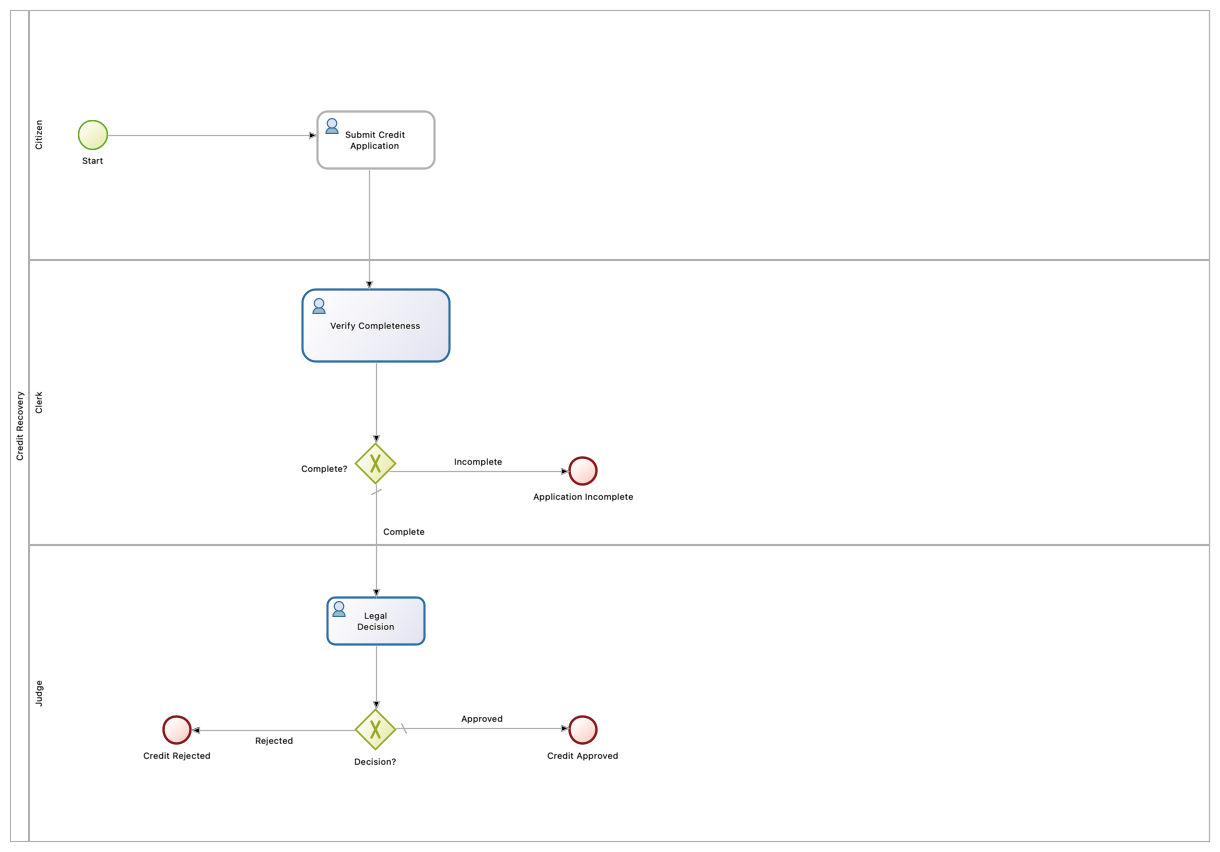
\includegraphics[width=0.95\textwidth]{figures/contest2_bpmn.png}
\caption{Contest 2 BPMN Diagram: Three-lane credit recovery process showing Citizen, Clerk, and Judge lanes with XOR gateways for completeness check and decision routing.}
\label{fig:contest2_bpmn}
\end{figure}

\begin{table}[H]
\centering
\caption{Contest 2: BPMN Element Summary}
\begin{tabular}{llp{6cm}}
\toprule
\textbf{Element Type} & \textbf{Name} & \textbf{Description} \\
\midrule
Start Event & Process Start & Initiates credit recovery process \\
Human Task & Submit Credit Application & Citizen enters credit claim details \\
Human Task & Verify Completeness & Clerk reviews application completeness \\
Human Task & Legal Decision & Judge decides on credit claim \\
XOR Gateway & Completeness Check & Routes based on isComplete \\
XOR Gateway & Decision Check & Routes based on decision \\
End Event & Application Incomplete & Terminates due to incomplete submission \\
End Event & Credit Rejected & Judge rejected the claim \\
End Event & Credit Approved & Judge approved the claim \\
\bottomrule
\end{tabular}
\label{tab:contest2_elements}
\end{table}

\subsection{Actors and Responsibilities}

\begin{table}[H]
\centering
\caption{Contest 2: Actor Responsibilities}
\begin{tabular}{llp{6cm}}
\toprule
\textbf{Lane} & \textbf{Actor} & \textbf{Responsibilities} \\
\midrule
Lane 1 & Citizen & Submits credit claim application with all required documentation \\
Lane 2 & Clerk & Reviews application for completeness and formal requirements \\
Lane 3 & Judge & Makes legal decision to approve or reject the credit claim \\
\bottomrule
\end{tabular}
\label{tab:contest2_actors}
\end{table}

\subsection{Business Data Model}

The CreditApplication business object contains 19 attributes covering creditor information, debtor information, credit details, and decision tracking:

\begin{figure}[H]
\centering
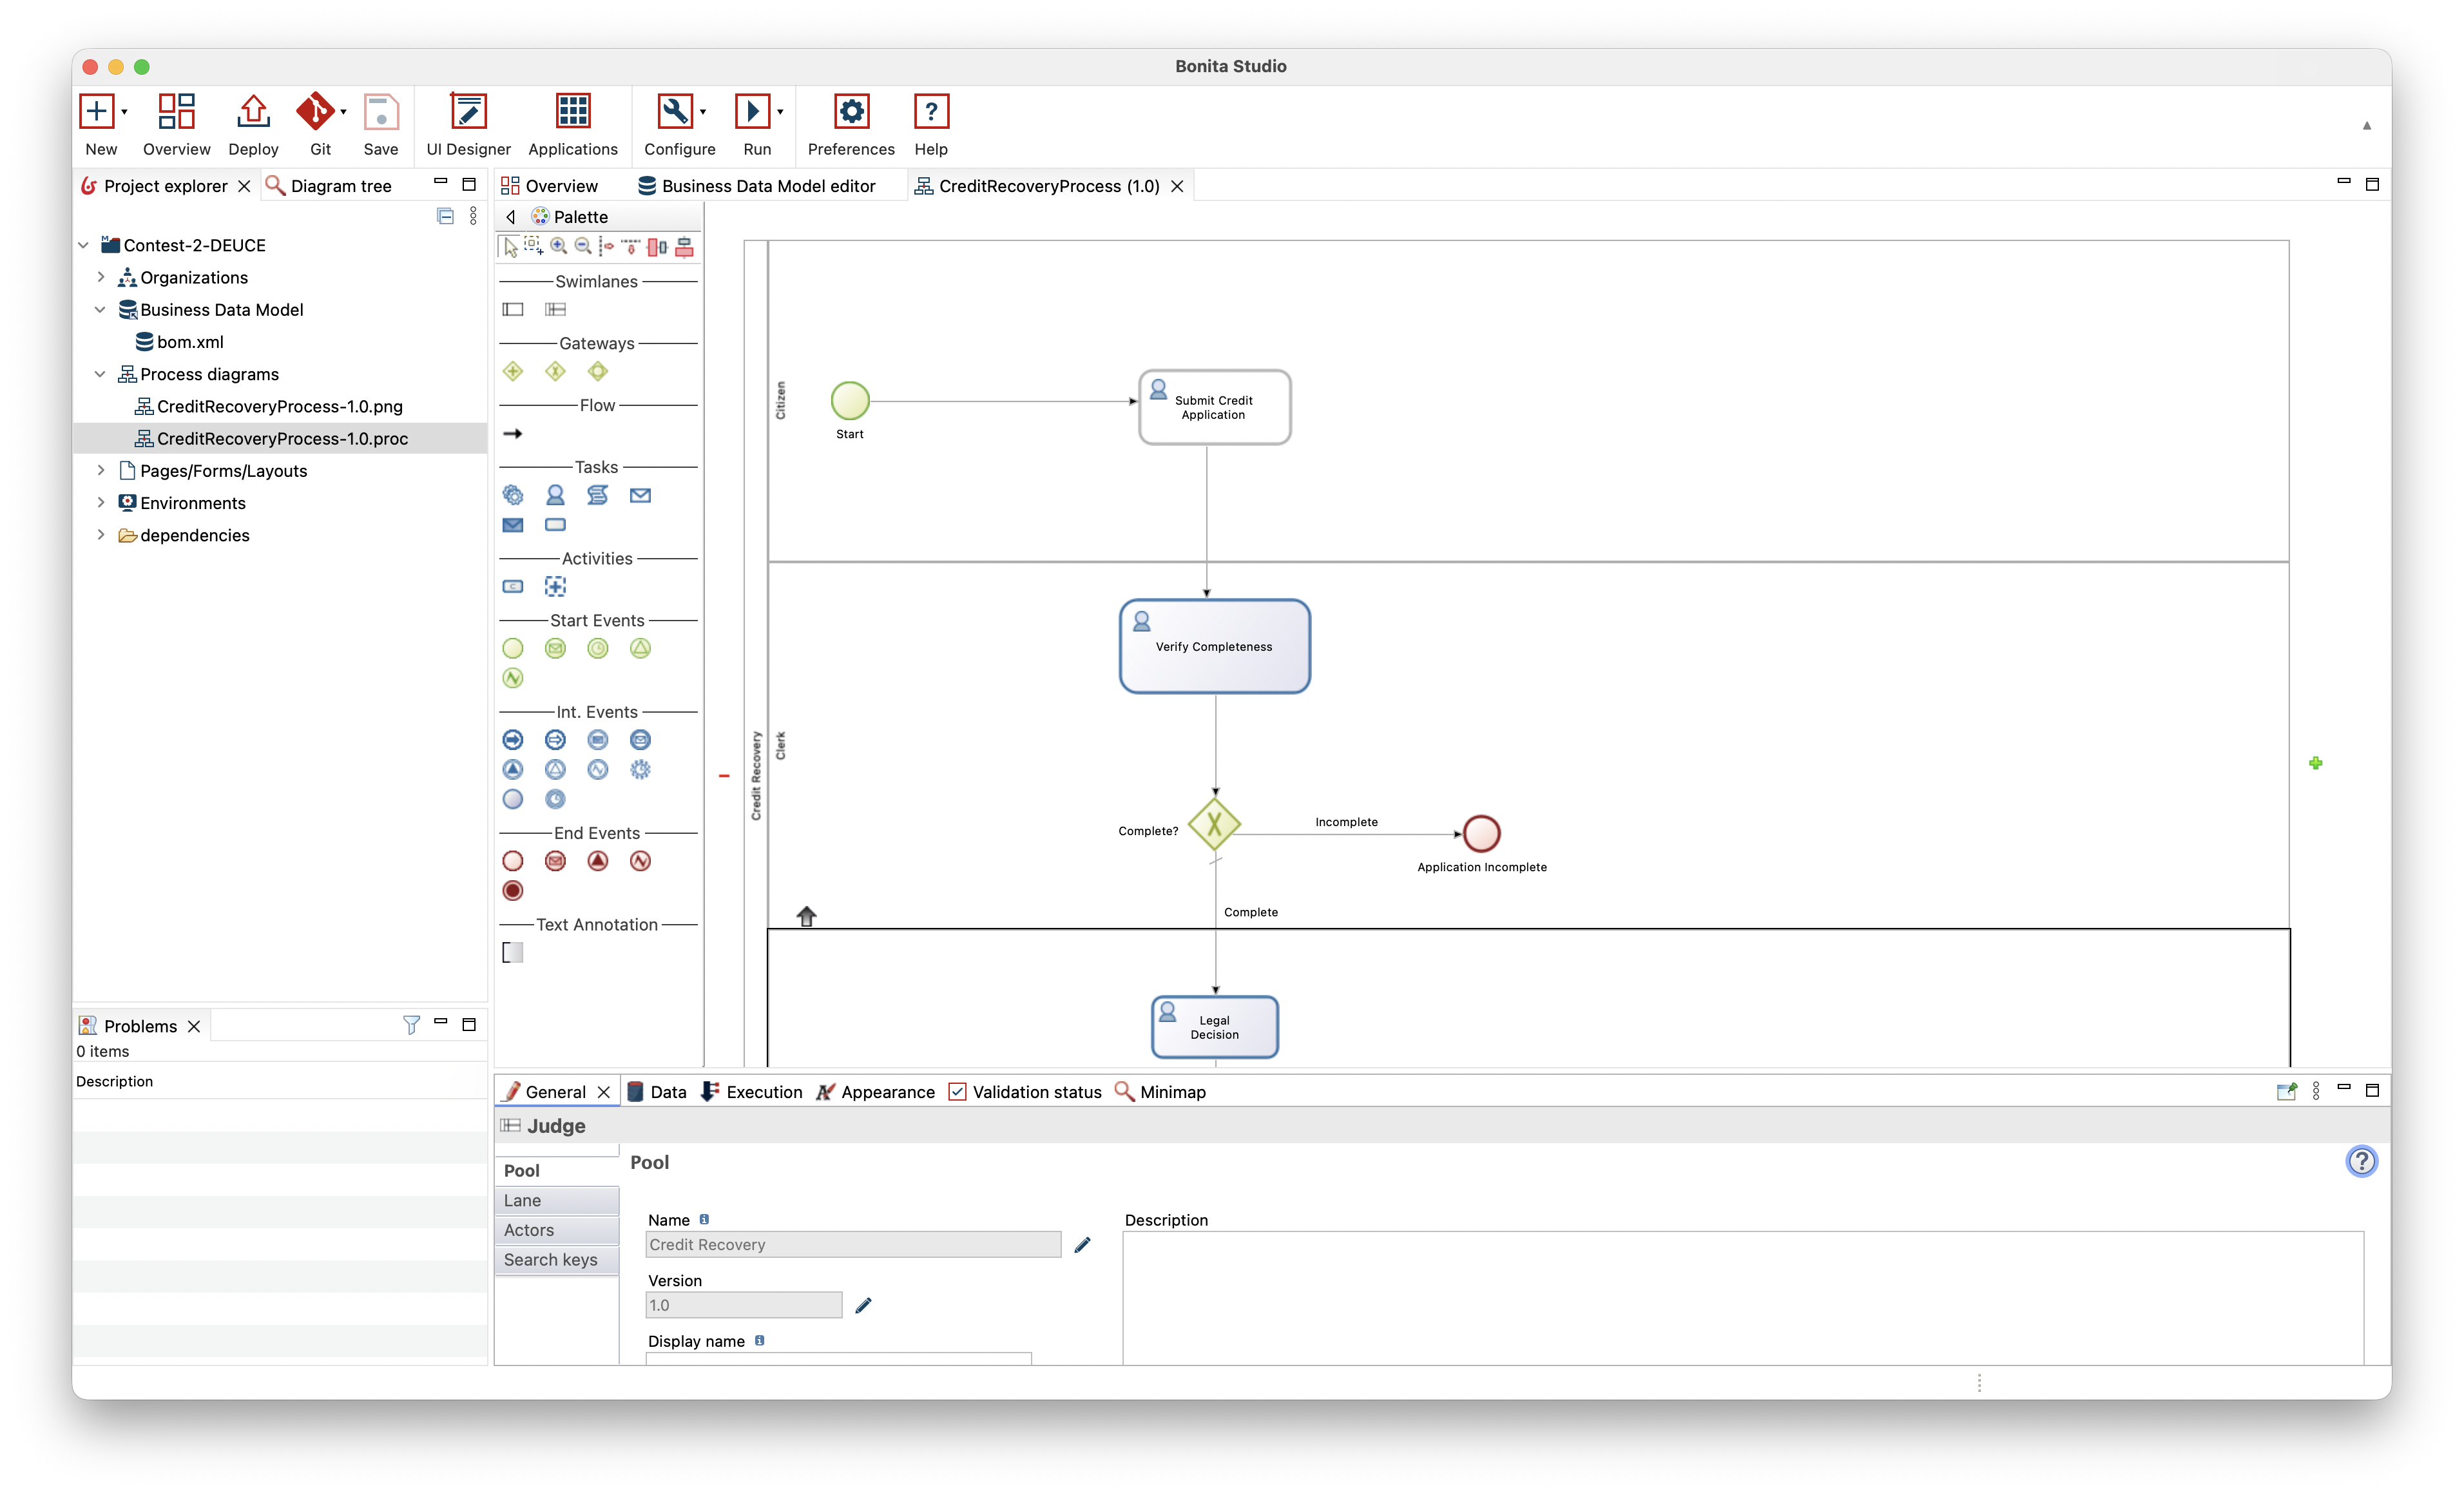
\includegraphics[width=0.85\textwidth]{figures/contest2_bdm.png}
\caption{Contest 2 BDM Editor: CreditApplication business object with 19 attributes defined in Bonita Studio's Business Data Model editor.}
\label{fig:contest2_bdm}
\end{figure}

\begin{longtable}{llcp{4cm}}
\caption{CreditApplication BDM Attributes} \label{tab:contest2_bdm} \\
\toprule
\textbf{Attribute} & \textbf{Type} & \textbf{Required} & \textbf{Description} \\
\midrule
\endfirsthead
\toprule
\textbf{Attribute} & \textbf{Type} & \textbf{Required} & \textbf{Description} \\
\midrule
\endhead
\midrule
\multicolumn{4}{r}{\textit{Continued on next page}} \\
\endfoot
\bottomrule
\endlastfoot
creditorName & STRING & Yes & Full name of the creditor \\
creditorEmail & STRING & Yes & Email address of the creditor \\
creditorPhone & STRING & Yes & Phone number of the creditor \\
creditorAddress & TEXT & Yes & Full address of the creditor \\
creditorCountry & STRING & Yes & Country of the creditor (EU) \\
debtorName & STRING & Yes & Full name of the debtor \\
debtorAddress & TEXT & Yes & Full address of the debtor \\
debtorCountry & STRING & Yes & Country of the debtor (EU) \\
creditAmount & DOUBLE & Yes & Amount of credit in EUR \\
creditDescription & TEXT & Yes & Description of the credit/debt \\
creditDate & DATE & Yes & Date when credit was issued \\
dueDate & DATE & Yes & Payment due date \\
additionalNotes & TEXT & No & Additional notes from citizen \\
isComplete & BOOLEAN & No & Completeness status \\
incompleteReason & TEXT & No & Reason for incompleteness \\
clerkNotes & TEXT & No & Notes from clerk review \\
decision & STRING & No & Judge's decision \\
decisionReason & TEXT & No & Rationale for the decision \\
judgeNotes & TEXT & No & Additional notes from judge \\
\end{longtable}

\subsection{Form Design}

Three distinct forms handle the workflow stages, each with appropriate read-only and editable sections:

\subsubsection{Citizen Form: Credit Application}

\begin{figure}[H]
\centering
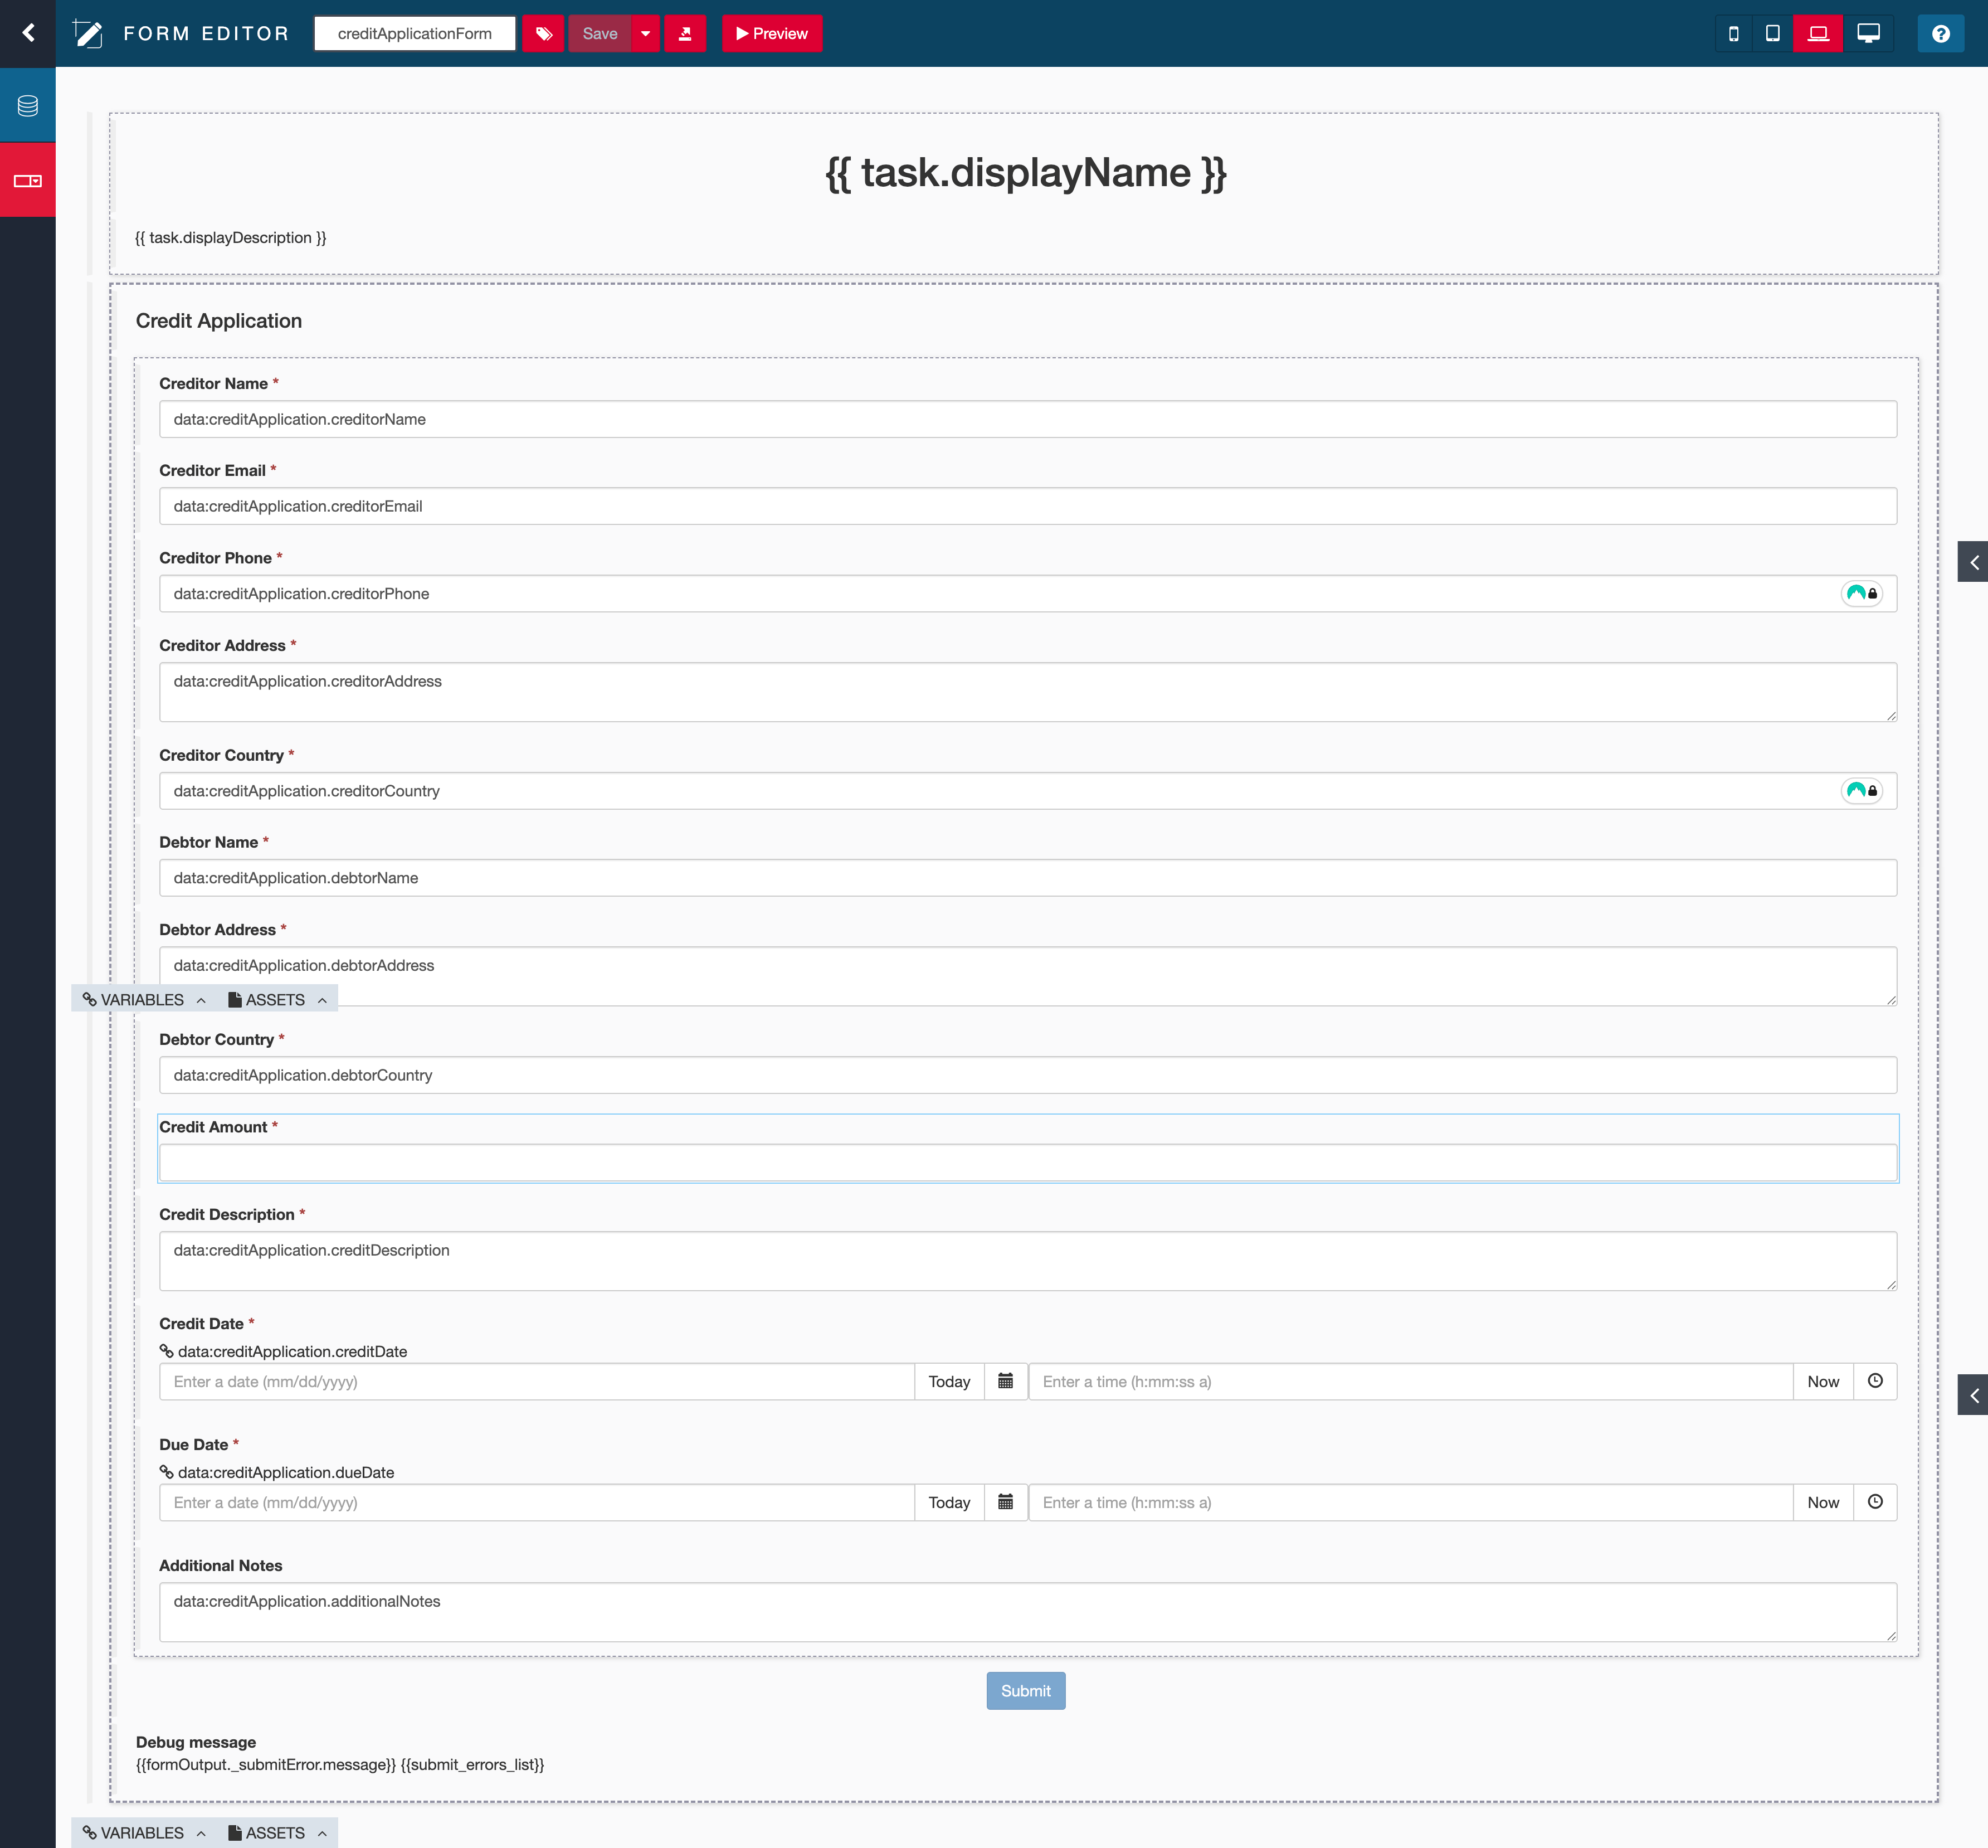
\includegraphics[width=0.85\textwidth]{figures/form_citizen.png}
\caption{Citizen Form: Editable form with 13 input fields for credit claim submission including creditor details, debtor details, and credit information.}
\label{fig:form_citizen}
\end{figure}

\begin{table}[H]
\centering
\caption{Citizen Form Fields}
\begin{tabular}{lllc}
\toprule
\textbf{Field} & \textbf{Label} & \textbf{Widget} & \textbf{Required} \\
\midrule
creditorName & Creditor Full Name & Text Input & Yes \\
creditorEmail & Creditor Email & Text Input & Yes \\
creditorPhone & Creditor Phone & Text Input & Yes \\
creditorAddress & Creditor Address & Text Area & Yes \\
creditorCountry & Creditor Country & Dropdown & Yes \\
debtorName & Debtor Full Name & Text Input & Yes \\
debtorAddress & Debtor Address & Text Area & Yes \\
debtorCountry & Debtor Country & Dropdown & Yes \\
creditAmount & Credit Amount (EUR) & Number Input & Yes \\
creditDescription & Credit Description & Text Area & Yes \\
creditDate & Original Credit Date & Date Picker & Yes \\
dueDate & Payment Due Date & Date Picker & Yes \\
additionalNotes & Additional Notes & Text Area & No \\
\bottomrule
\end{tabular}
\label{tab:citizen_form}
\end{table}

\subsubsection{Clerk Form: Completeness Verification}

\begin{figure}[H]
\centering
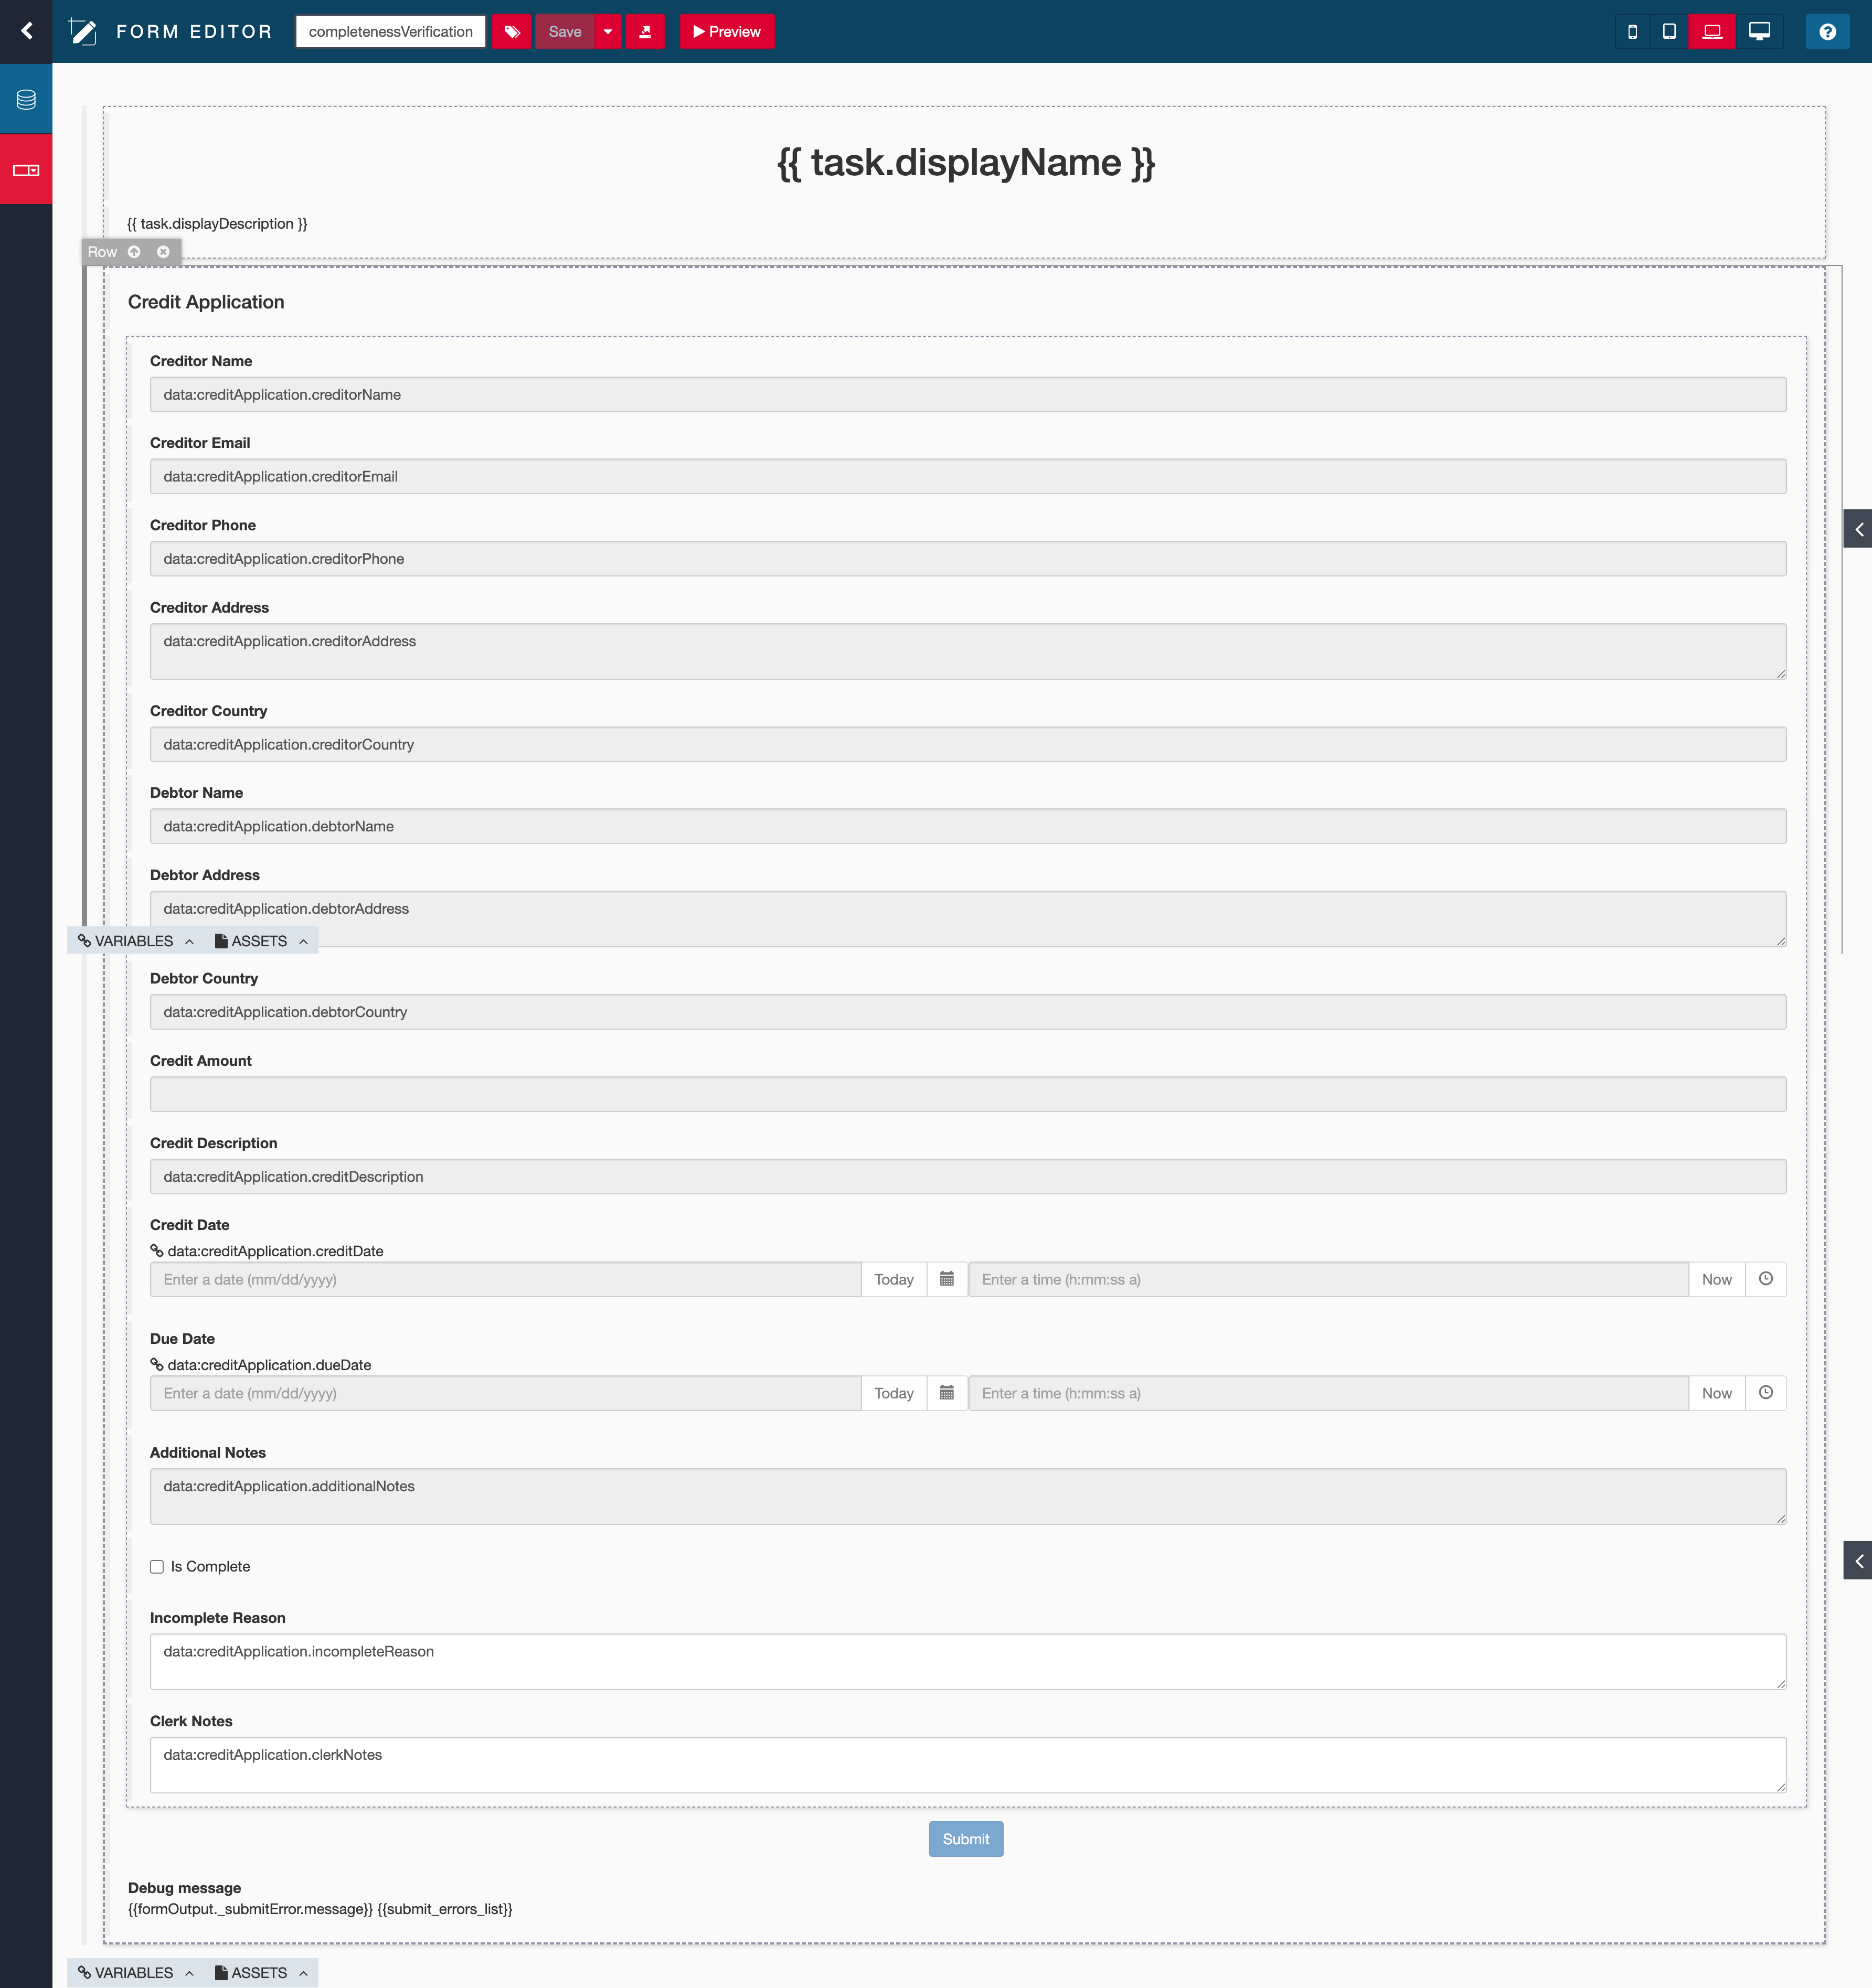
\includegraphics[width=0.85\textwidth]{figures/form_clerk.png}
\caption{Clerk Form: Read-only display of application data with editable decision section for completeness verification.}
\label{fig:form_clerk}
\end{figure}

The clerk form displays all citizen-submitted data in read-only mode, with an editable section for:
\begin{itemize}
    \item \texttt{isComplete}: Radio button (Yes/No)
    \item \texttt{incompleteReason}: Text area (required if isComplete = No)
    \item \texttt{clerkNotes}: Text area for internal notes
\end{itemize}

\subsubsection{Judge Form: Legal Decision}

\begin{figure}[H]
\centering
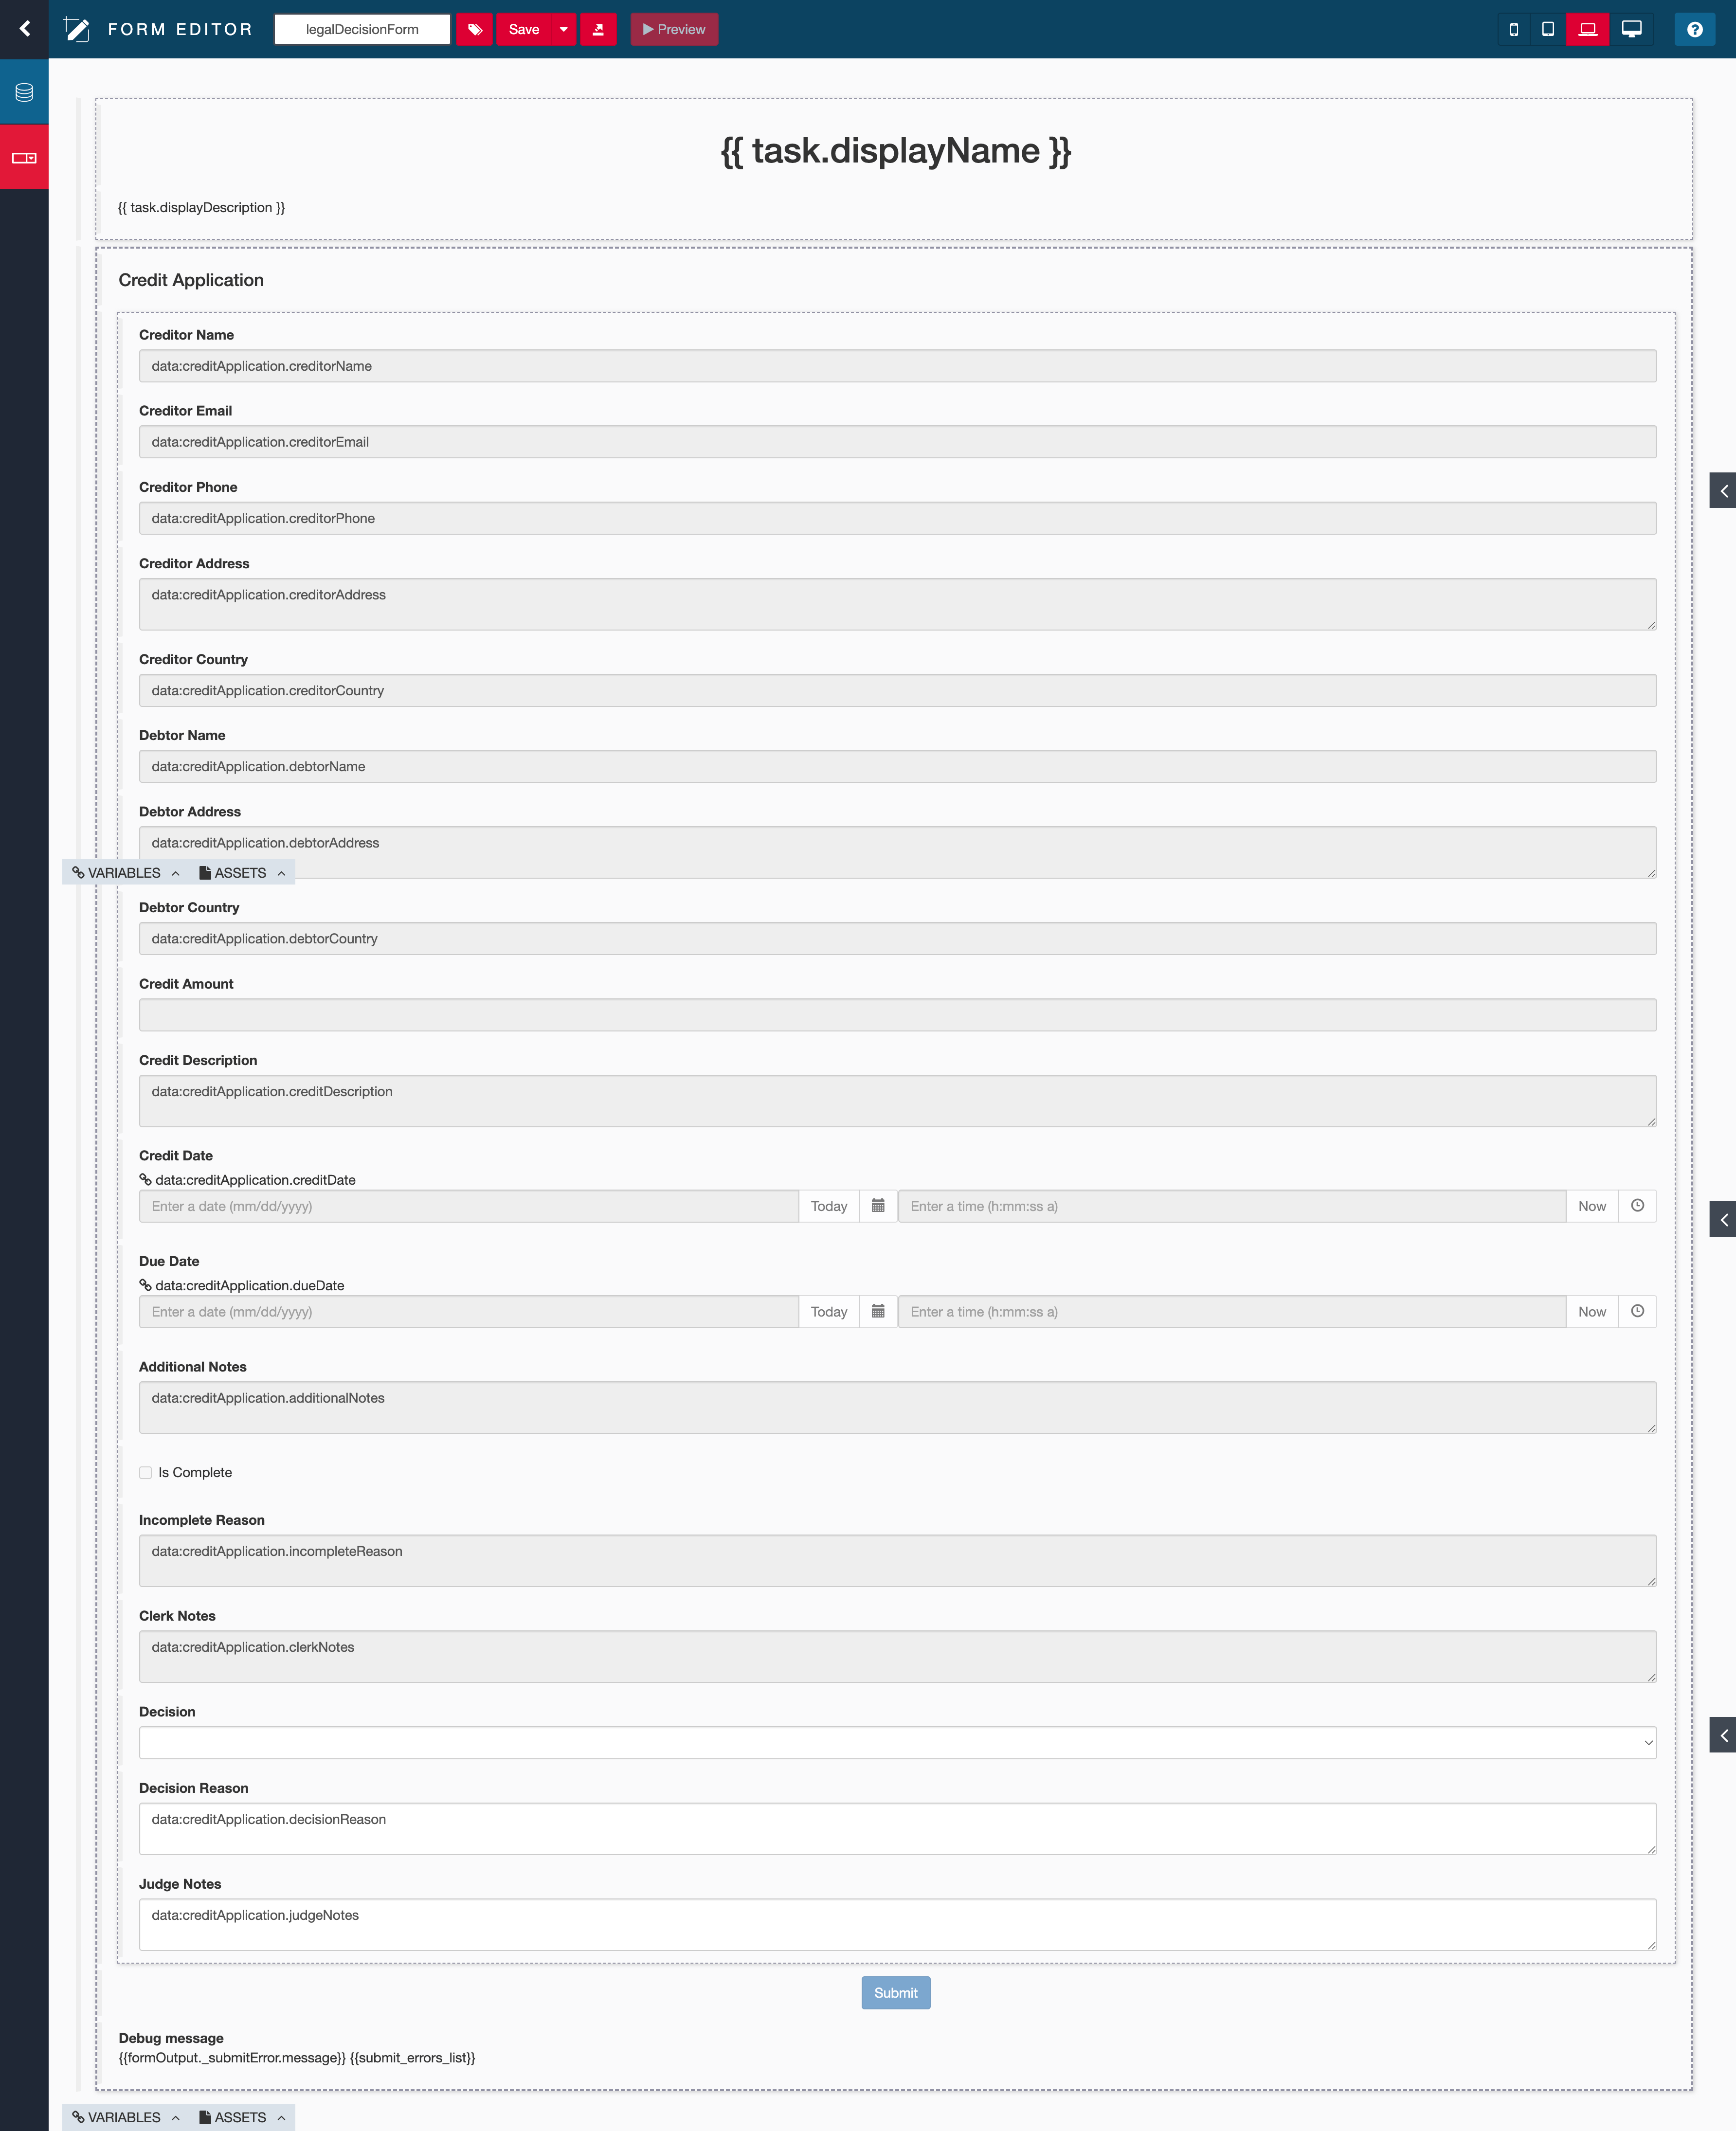
\includegraphics[width=0.85\textwidth]{figures/form_judge.png}
\caption{Judge Form: Read-only display of application and clerk notes with editable decision section for legal ruling.}
\label{fig:form_judge}
\end{figure}

The judge form displays application data and clerk notes in read-only mode, with editable fields for:
\begin{itemize}
    \item \texttt{decision}: Dropdown (Approved/Rejected)
    \item \texttt{decisionReason}: Text area (required)
    \item \texttt{judgeNotes}: Text area for additional notes
\end{itemize}

\subsection{Gateway Logic}

Two XOR gateways control process flow based on business data:

\begin{lstlisting}[language=Java, caption=Contest 2 Gateway Conditions (Groovy)]
// Gateway 1: Completeness Check
// Condition for "Complete" flow
creditApplication.isComplete == true
// Default flow: Application Incomplete (End Event)

// Gateway 2: Decision Check
// Condition for "Approved" flow
creditApplication.decision == "Approved"
// Default flow: Credit Rejected (End Event)
\end{lstlisting}

\section{Contest 3: IDEA Labor Disputes}

\subsection{Business Context}

IDEA (Intelligent Digitization for European Access to justice) focuses on predictive justice and digitization in labor law. The project addresses:

\begin{itemize}
    \item \textbf{Digital Journey}: Guiding citizens from dispute perception to resolution
    \item \textbf{Procedure Selection}: Choice between assisted negotiation and judicial appeal
    \item \textbf{AI and Big Data}: Using predictive analytics while respecting fundamental rights
\end{itemize}

The implemented workflow allows workers to describe disputes and indicate preferences, with office review and confirmation before case preparation.

\subsection{Process Architecture}

The IDEA process implements a two-lane architecture with a branching structure after review:

\begin{figure}[H]
\centering
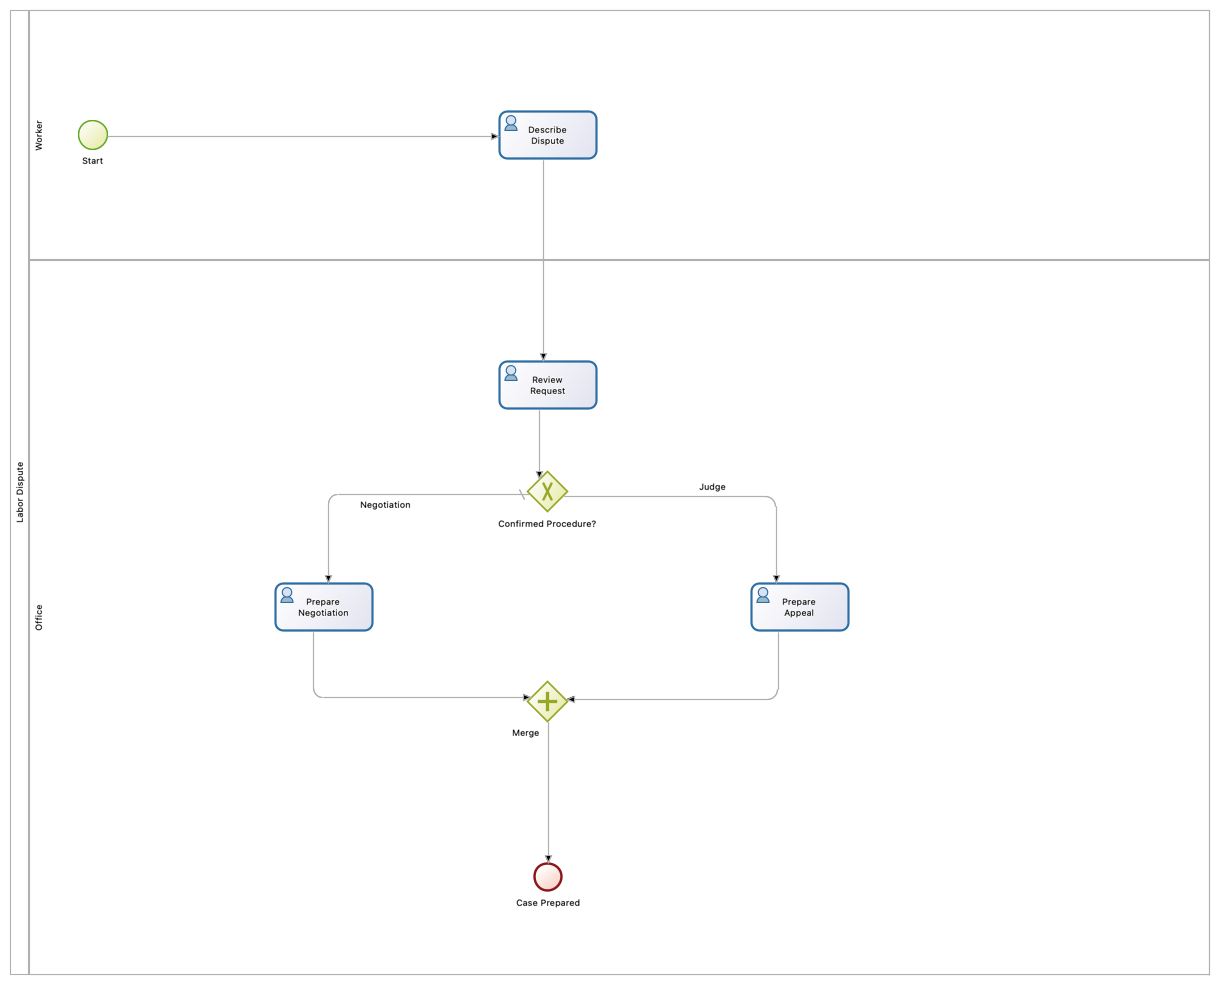
\includegraphics[width=0.95\textwidth]{figures/contest3_bpmn.png}
\caption{Contest 3 BPMN Diagram: Two-lane labor dispute process showing Worker and Office lanes with XOR gateway for procedure selection and merge before single end event.}
\label{fig:contest3_bpmn}
\end{figure}

\begin{table}[H]
\centering
\caption{Contest 3: BPMN Element Summary}
\begin{tabular}{llp{6cm}}
\toprule
\textbf{Element Type} & \textbf{Name} & \textbf{Description} \\
\midrule
Start Event & Process Start & Initiates labor dispute process \\
Human Task & Describe Dispute & Worker describes issue and preference \\
Human Task & Review Request & Office reviews and confirms procedure \\
Human Task & Prepare Negotiation & Office prepares negotiation case \\
Human Task & Prepare Appeal & Office prepares court appeal \\
XOR Gateway & Procedure Selection & Routes based on confirmedProcedure \\
Merge Gateway & Flow Merge & Converges paths before end \\
End Event & Case Prepared & Single unified end event \\
\bottomrule
\end{tabular}
\label{tab:contest3_elements}
\end{table}

\subsection{Key Design Feature: Preference vs Confirmation}

A distinctive feature of Contest 3 is the dual-tracking of procedure preferences:

\begin{table}[H]
\centering
\caption{Preference vs Confirmation Tracking}
\begin{tabular}{lll}
\toprule
\textbf{Variable} & \textbf{Set By} & \textbf{Purpose} \\
\midrule
preferredProcedure & Worker & Initial worker preference \\
confirmedProcedure & Office & Final office decision \\
overrideReason & Office & Required if procedures differ \\
\bottomrule
\end{tabular}
\label{tab:preference_tracking}
\end{table}

This design enables:
\begin{itemize}
    \item Explicit tracking of worker's initial preference
    \item Documentation of office's decision-making process
    \item Analysis of override patterns for process improvement
    \item Transparency and accountability in procedure selection
\end{itemize}

\subsection{Actors and Responsibilities}

\begin{table}[H]
\centering
\caption{Contest 3: Actor Responsibilities}
\begin{tabular}{llp{7cm}}
\toprule
\textbf{Lane} & \textbf{Actor} & \textbf{Responsibilities} \\
\midrule
Lane 1 & Worker & Describes labor dispute and indicates preferred resolution procedure \\
Lane 2 & Office & Reviews requests, confirms appropriate procedure, and prepares cases \\
\bottomrule
\end{tabular}
\label{tab:contest3_actors}
\end{table}

\subsection{Business Data Model}

The LaborDispute business object contains 30 attributes organized into six categories:

\begin{figure}[H]
\centering
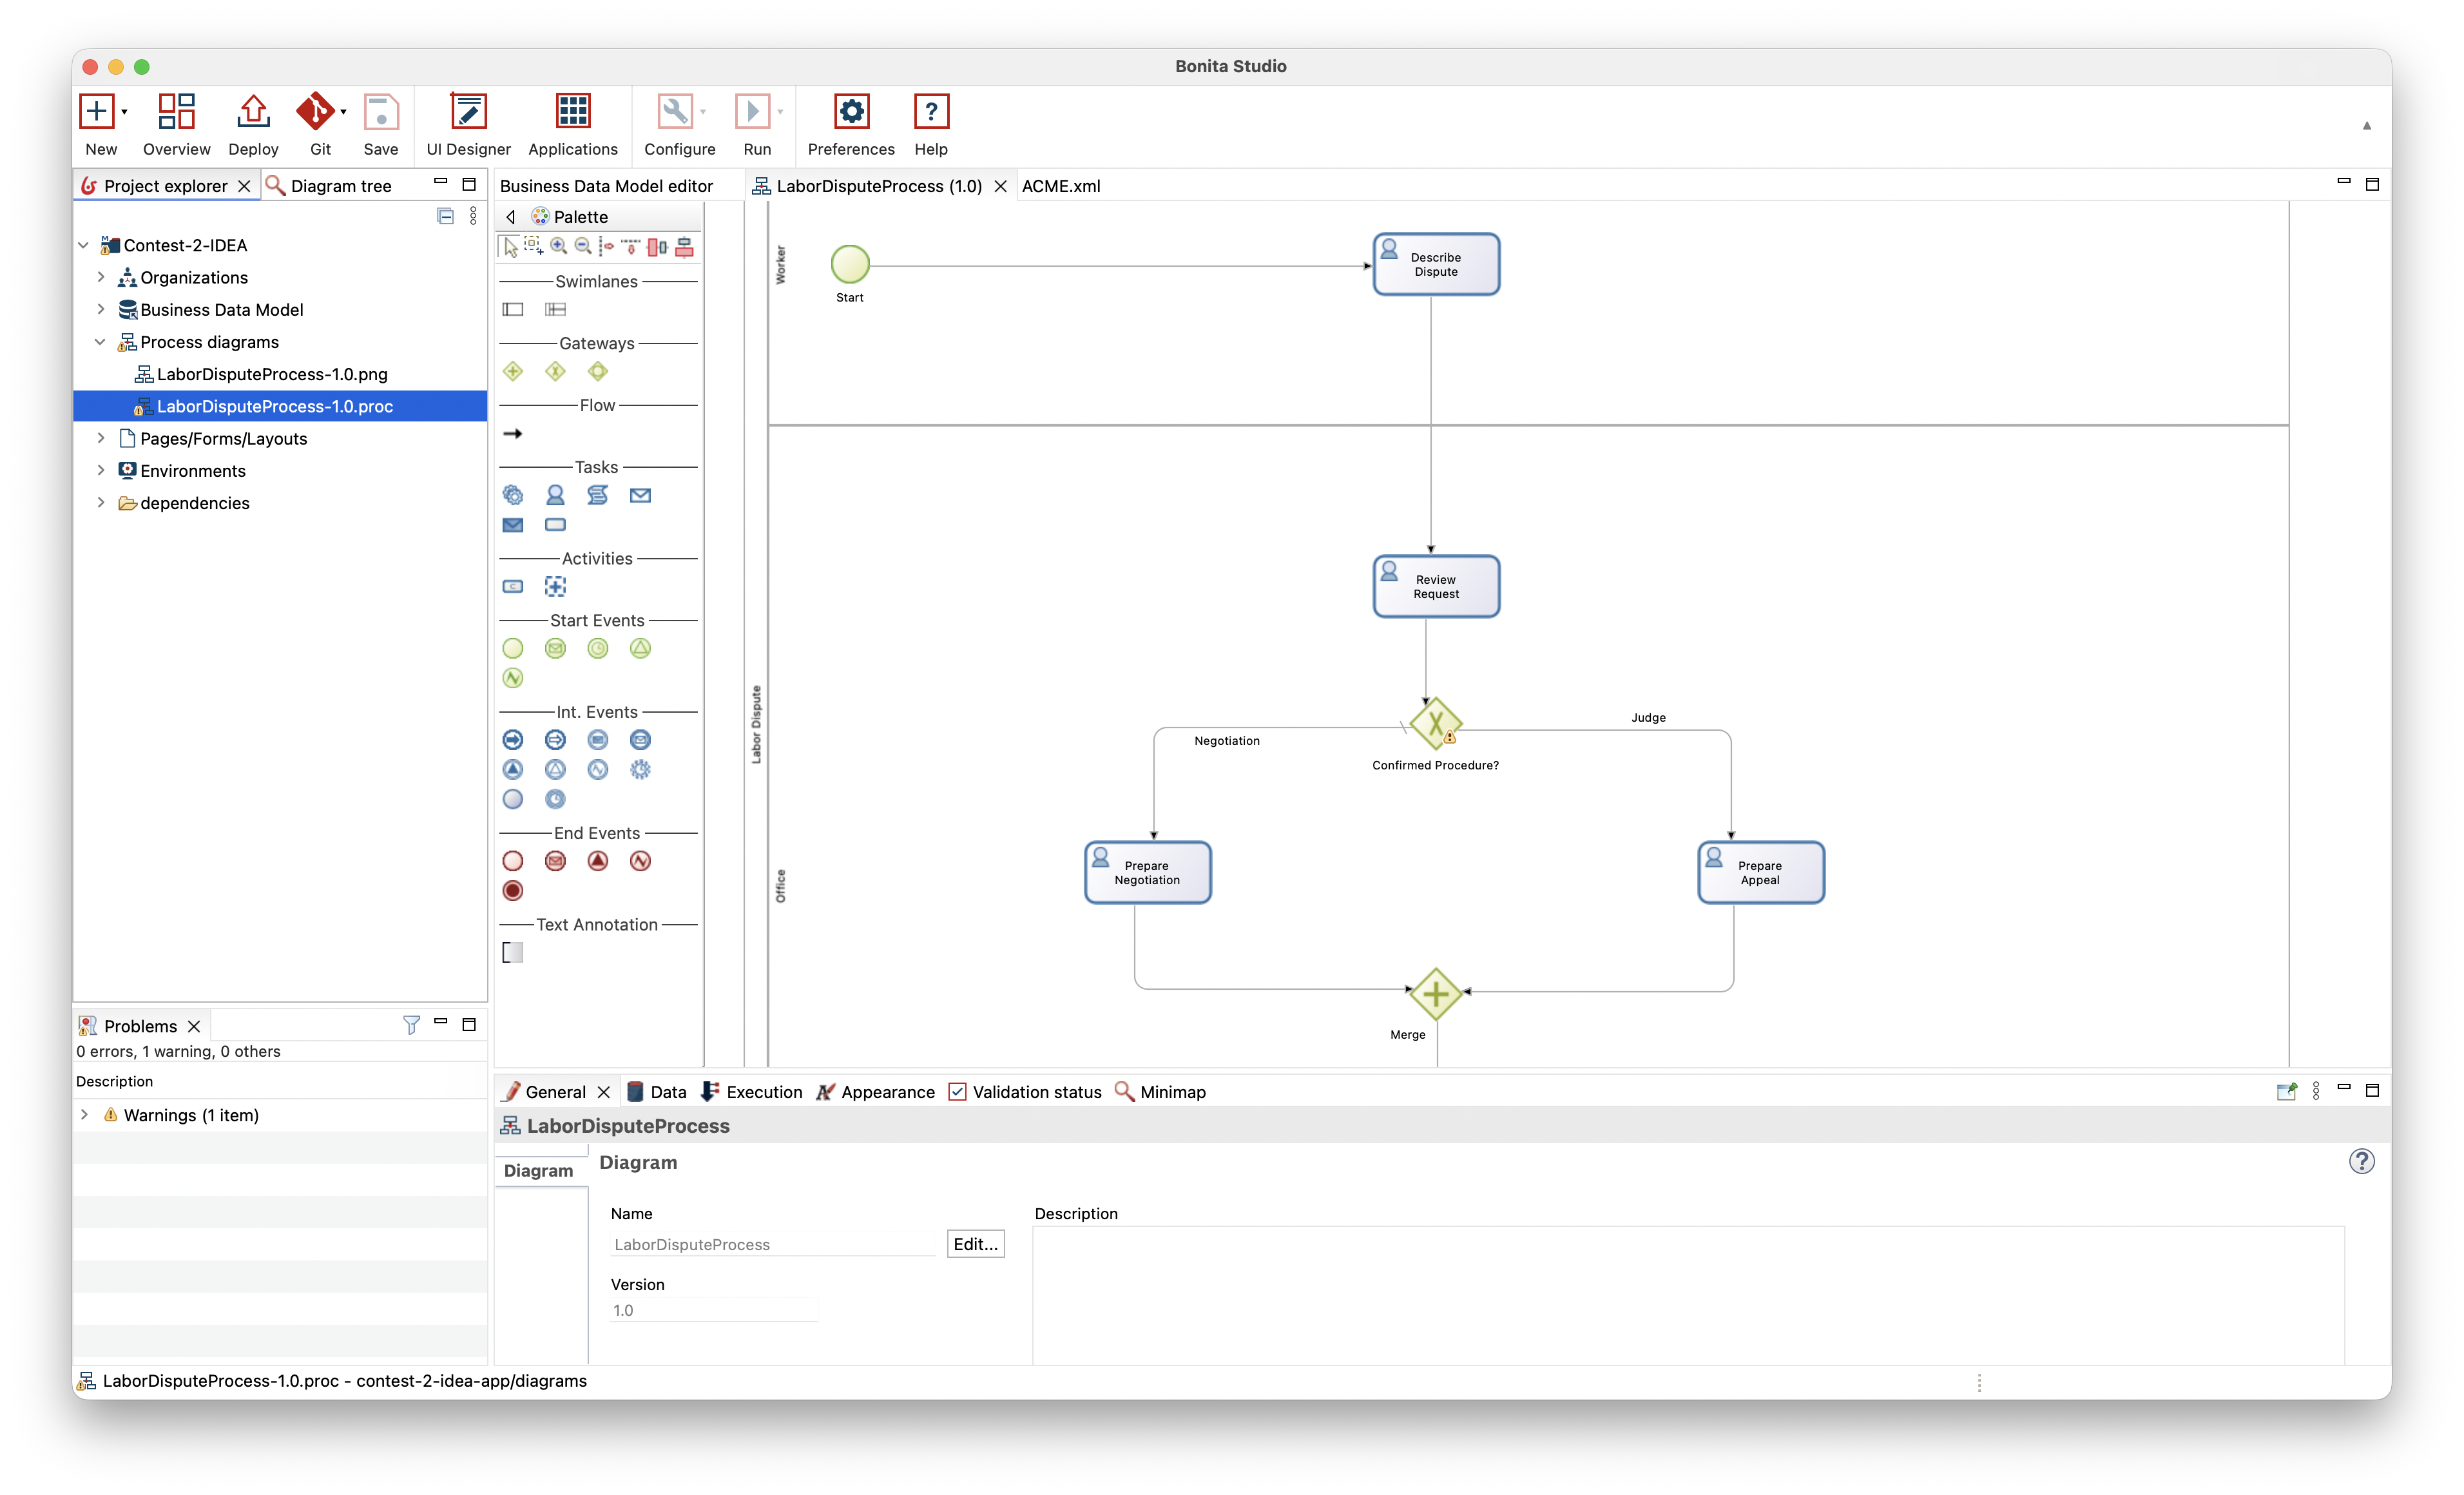
\includegraphics[width=0.85\textwidth]{figures/contest3_bdm.png}
\caption{Contest 3 BDM Editor: LaborDispute business object with 30 attributes covering worker information, employer details, dispute data, review decisions, and case preparation fields.}
\label{fig:contest3_bdm}
\end{figure}

\begin{longtable}{llcp{4cm}}
\caption{LaborDispute BDM Attributes} \label{tab:contest3_bdm} \\
\toprule
\textbf{Attribute} & \textbf{Type} & \textbf{Required} & \textbf{Category} \\
\midrule
\endfirsthead
\toprule
\textbf{Attribute} & \textbf{Type} & \textbf{Required} & \textbf{Category} \\
\midrule
\endhead
\midrule
\multicolumn{4}{r}{\textit{Continued on next page}} \\
\endfoot
\bottomrule
\endlastfoot
workerName & STRING & Yes & Worker Info \\
workerEmail & STRING & Yes & Worker Info \\
workerPhone & STRING & Yes & Worker Info \\
workerAddress & TEXT & Yes & Worker Info \\
employerName & STRING & Yes & Employer Info \\
employerAddress & TEXT & Yes & Employer Info \\
employmentStartDate & DATE & Yes & Employer Info \\
employmentEndDate & DATE & No & Employer Info \\
currentlyEmployed & BOOLEAN & Yes & Employer Info \\
disputeCategory & STRING & Yes & Dispute Details \\
disputeDescription & TEXT & Yes & Dispute Details \\
disputeDate & DATE & Yes & Dispute Details \\
desiredOutcome & TEXT & Yes & Dispute Details \\
preferredProcedure & STRING & Yes & Dispute Details \\
preferenceReason & TEXT & No & Dispute Details \\
confirmedProcedure & STRING & No & Review Decision \\
overrideReason & TEXT & No & Review Decision \\
caseComplexity & STRING & No & Review Decision \\
priorityLevel & STRING & No & Review Decision \\
officeNotes & TEXT & No & Review Decision \\
caseFileNumber & STRING & No & Case Preparation \\
negotiationType & STRING & No & Negotiation Fields \\
scheduledDate & DATE & No & Negotiation Fields \\
negotiationMode & STRING & No & Negotiation Fields \\
mediatorRequired & BOOLEAN & No & Negotiation Fields \\
courtType & STRING & No & Appeal Fields \\
filingDate & DATE & No & Appeal Fields \\
legalRepRequired & BOOLEAN & No & Appeal Fields \\
courtFees & DOUBLE & No & Appeal Fields \\
appealSummary & TEXT & No & Appeal Fields \\
\end{longtable}

\subsection{Form Design}

Four forms handle the workflow stages:

\subsubsection{Worker Form: Dispute Description}

\begin{figure}[H]
\centering
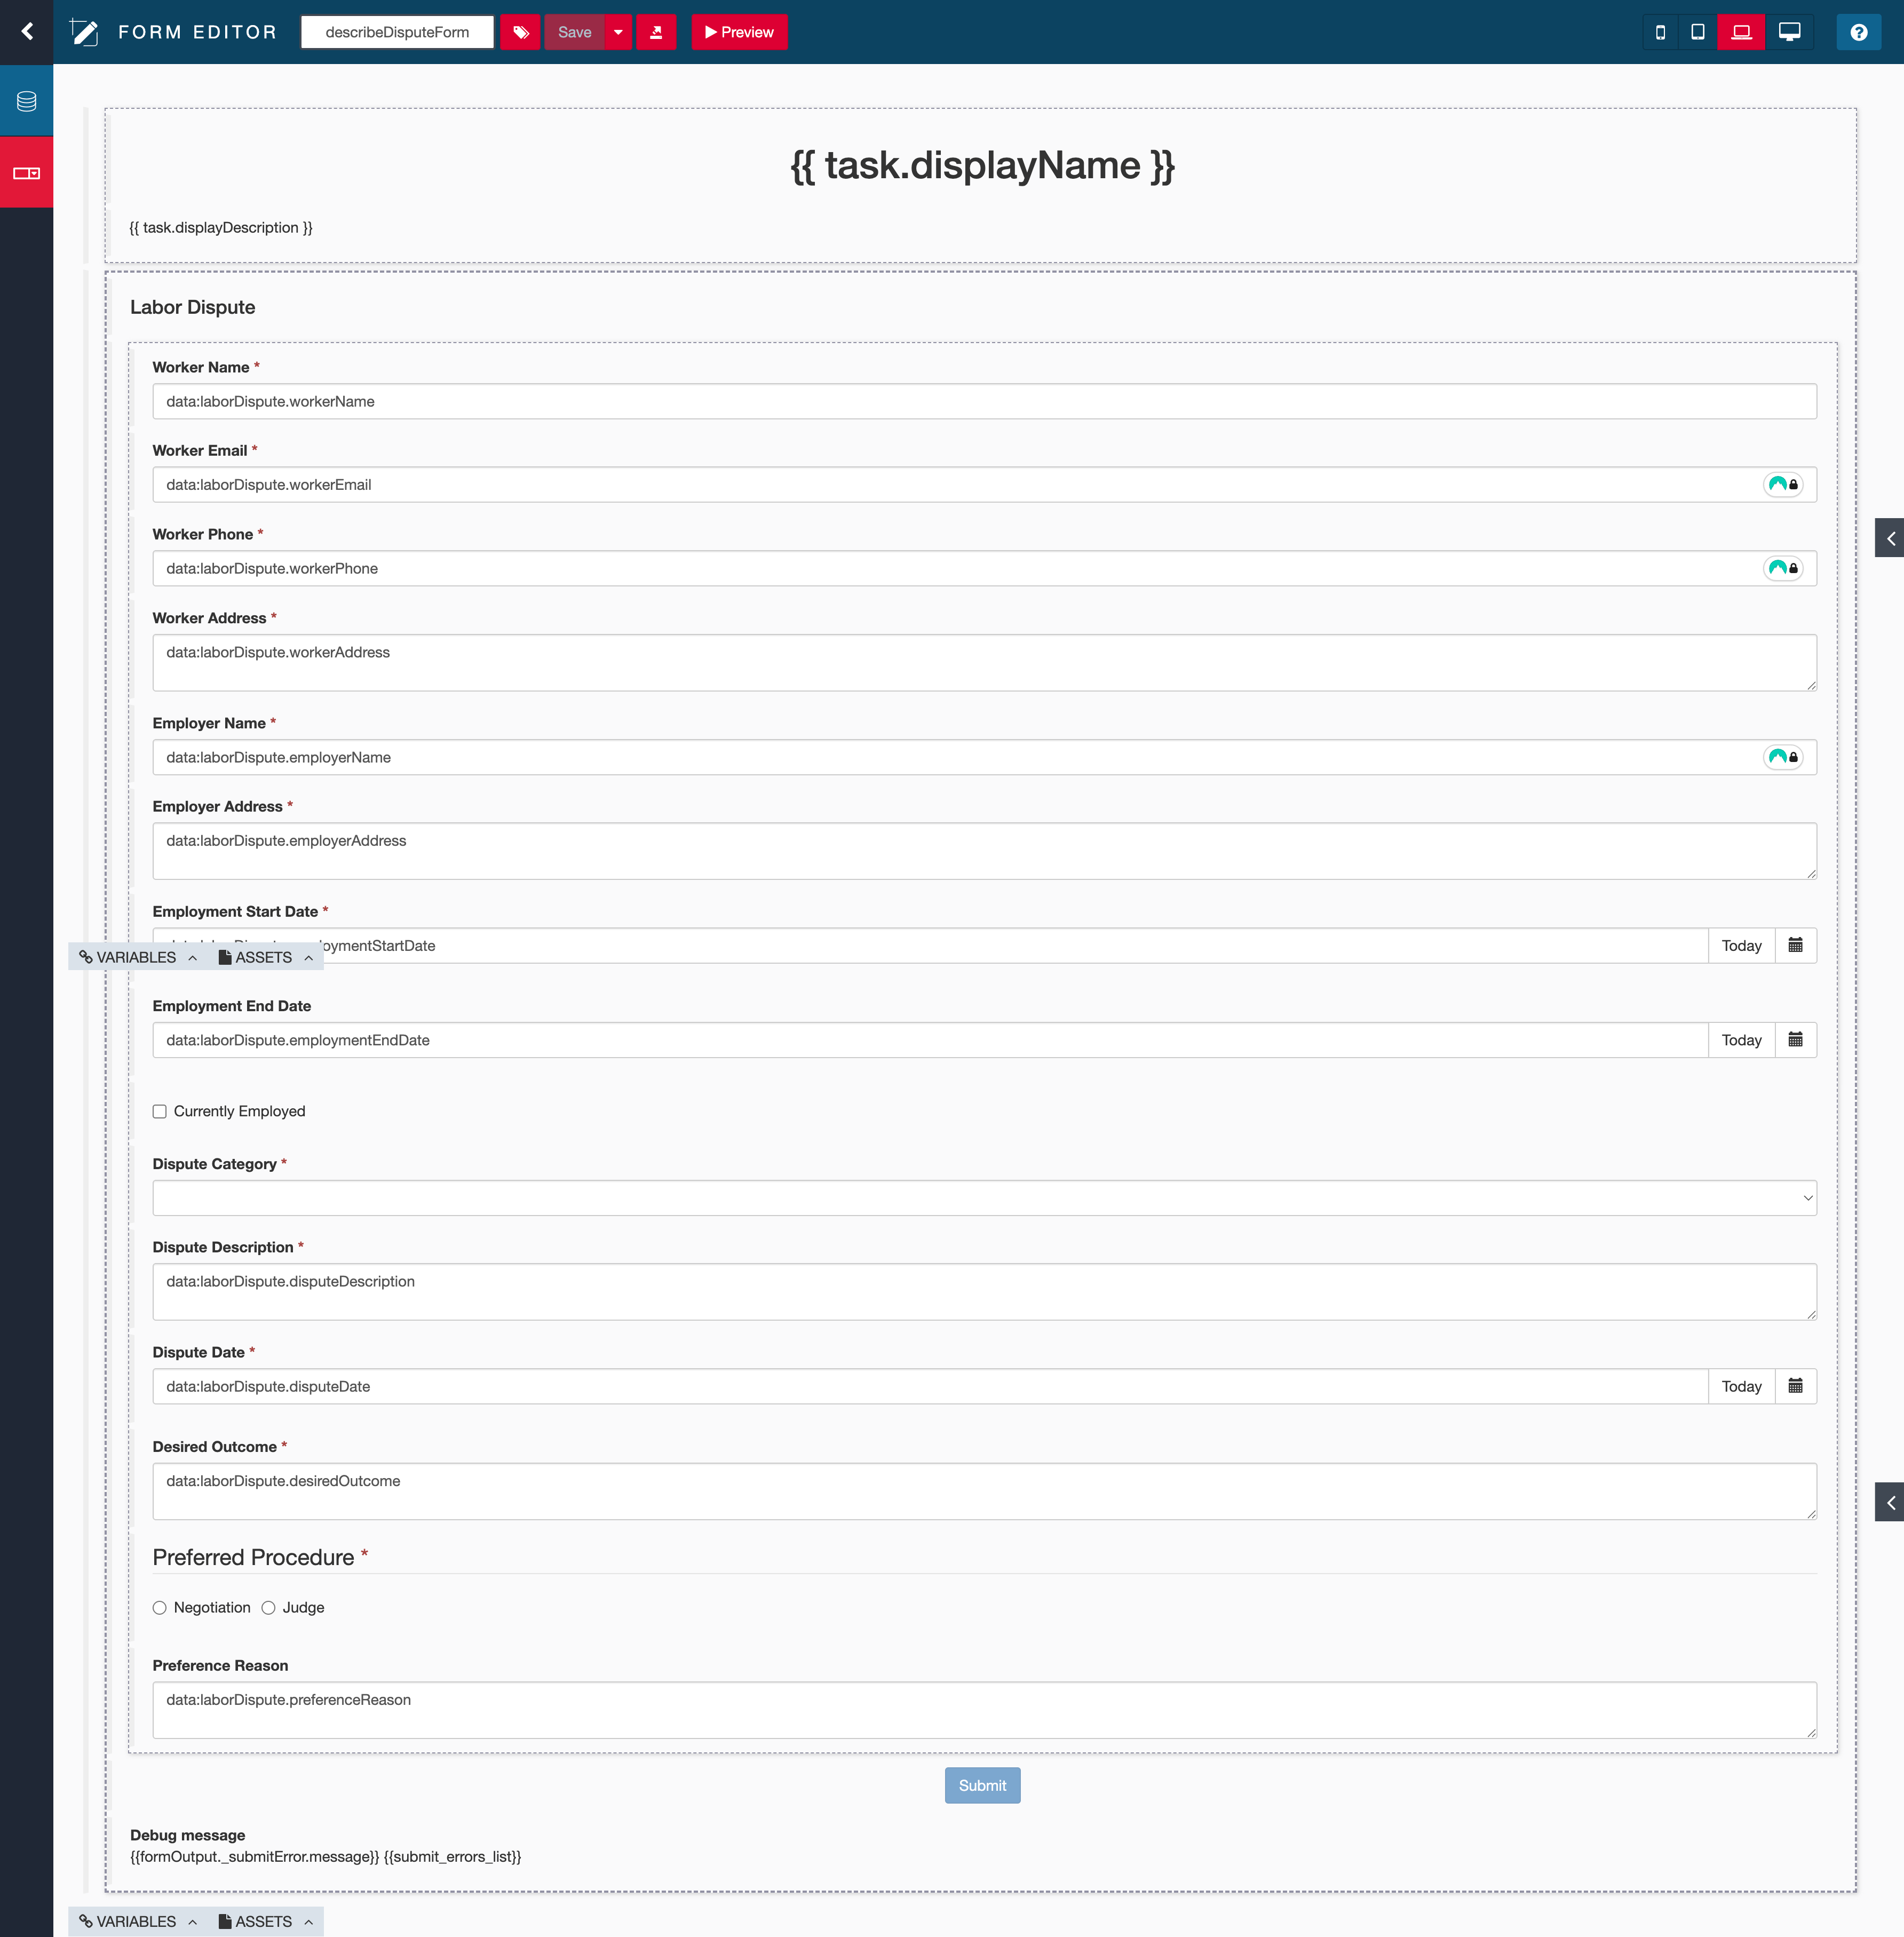
\includegraphics[width=0.85\textwidth]{figures/form_worker.png}
\caption{Worker Form: Editable form for dispute description including personal details, employer information, dispute category, and procedure preference selection.}
\label{fig:form_worker}
\end{figure}

Key fields include:
\begin{itemize}
    \item Personal information (name, email, phone, address)
    \item Employment details (employer, dates, current status)
    \item Dispute information (category, description, desired outcome)
    \item \textbf{Procedure preference}: Radio button (Negotiation/Judge)
\end{itemize}

\textbf{Dispute Categories:}
\begin{itemize}
    \item Unfair Dismissal
    \item Wage Dispute
    \item Working Conditions
    \item Discrimination
    \item Harassment
    \item Contract Violation
    \item Benefits Dispute
    \item Other
\end{itemize}

\subsubsection{Office Form: Request Review}

\begin{figure}[H]
\centering
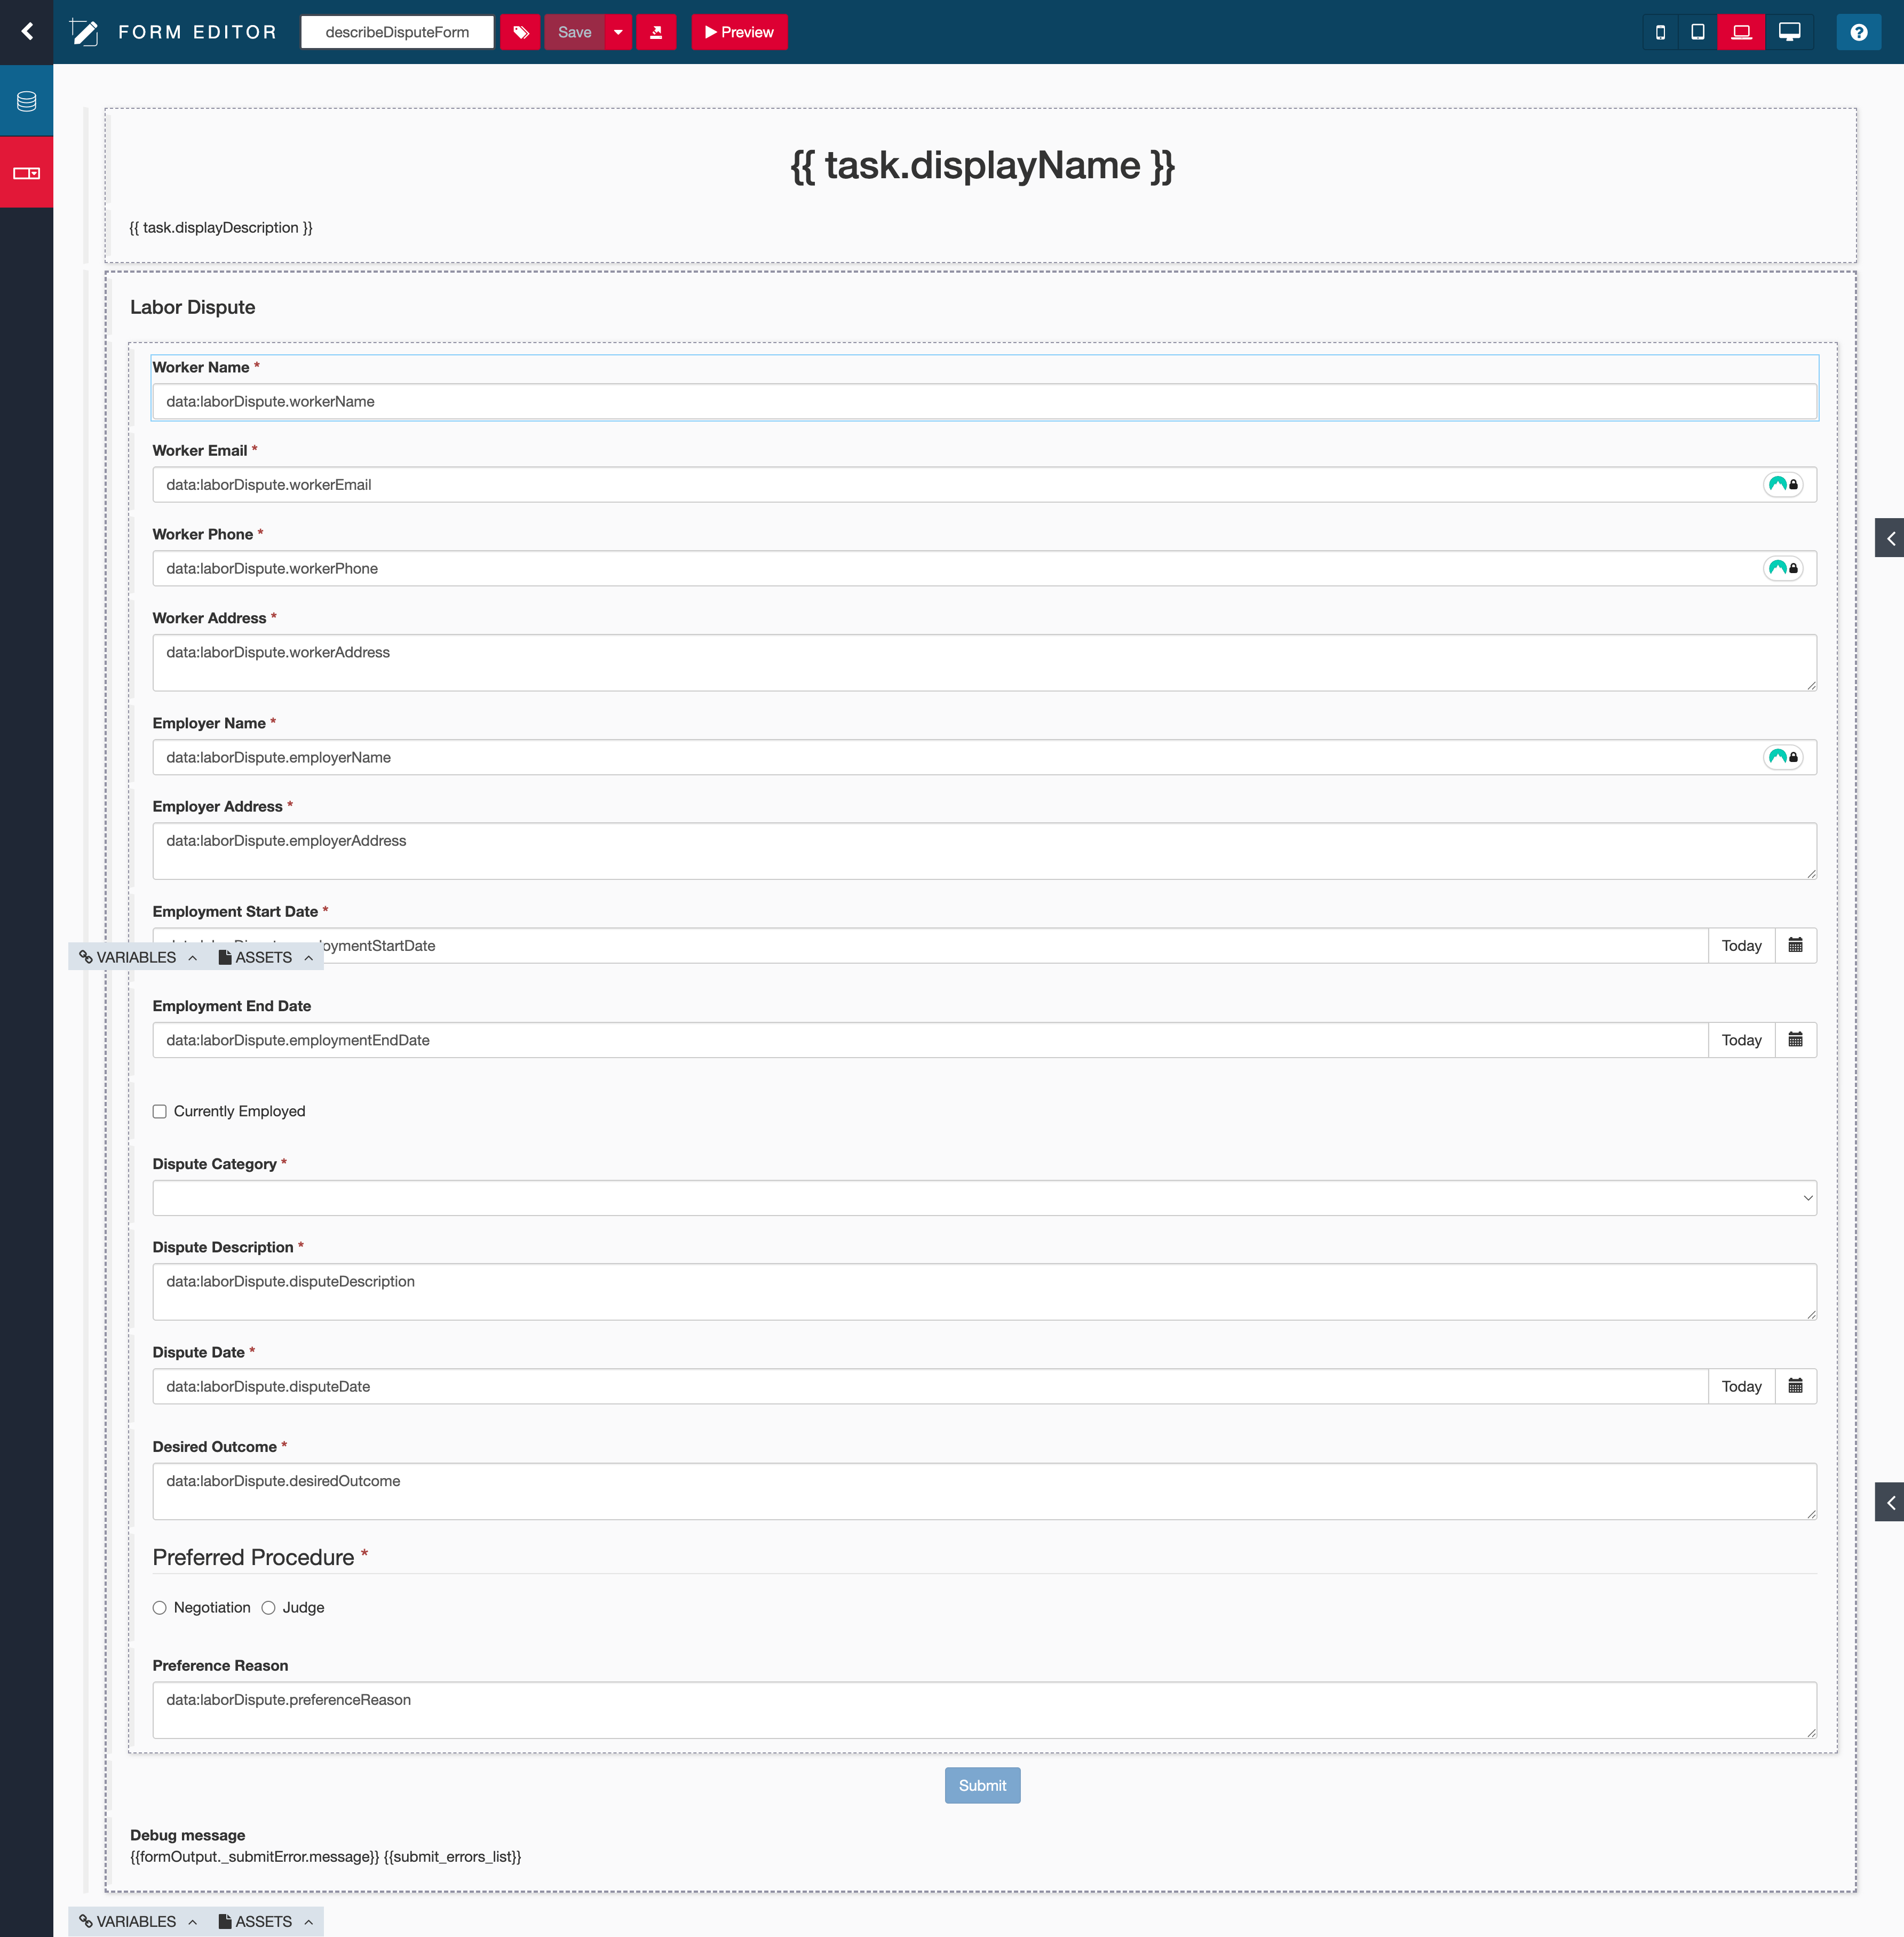
\includegraphics[width=0.85\textwidth]{figures/form_office.png}
\caption{Office Form: Read-only display of worker submission with editable section for procedure confirmation, complexity assessment, and priority assignment.}
\label{fig:form_office}
\end{figure}

The review form displays worker-submitted data in read-only mode, with editable fields for:
\begin{itemize}
    \item \texttt{confirmedProcedure}: Radio button (Negotiation/Judge)
    \item \texttt{overrideReason}: Text area (required if different from preference)
    \item \texttt{caseComplexity}: Dropdown (Low/Medium/High)
    \item \texttt{priorityLevel}: Dropdown (Normal/Urgent)
    \item \texttt{officeNotes}: Text area for internal notes
\end{itemize}

\subsubsection{Negotiation and Appeal Preparation Forms}

These forms provide procedure-specific fields for case preparation:

\begin{table}[H]
\centering
\caption{Preparation Form Fields}
\begin{tabular}{ll}
\toprule
\textbf{Negotiation Preparation} & \textbf{Appeal Preparation} \\
\midrule
Negotiation Type (Assisted/Automated) & Court Type (Labor Tribunal/Civil) \\
Scheduled Date & Filing Date \\
Scheduled Time & Hearing Preference \\
Mode (Online/In-Person) & Legal Rep Required \\
Mediator Required & Documents to File \\
Documents to Provide & Estimated Court Fees \\
Preparation Notes & Appeal Summary \\
\bottomrule
\end{tabular}
\label{tab:prep_forms}
\end{table}

\subsection{Gateway Logic}

A single XOR gateway controls the procedure branch:

\begin{lstlisting}[language=Java, caption=Contest 3 Gateway Condition (Groovy)]
// Gateway: Procedure Selection
// Condition for "Negotiation" flow
laborDispute.confirmedProcedure == "Negotiation"
// Default flow: Prepare Appeal
\end{lstlisting}

Note that the gateway uses \texttt{confirmedProcedure} (office's decision), not \texttt{preferredProcedure} (worker's choice).

\section{Technical Implementation}

\subsection{Actor Organization}

Both processes require organization structure setup in Bonita:

\begin{lstlisting}[caption=Organization Structure]
// Contest 2: DEUCE
Organization:
  +-- Citizen (Group: external_users)
  +-- Clerk (Group: court_staff)
  |     +-- Role: Administrative
  +-- Judge (Group: judiciary)
        +-- Role: Judicial Authority

// Contest 3: IDEA
Organization:
  +-- Worker (Group: external_users)
  |     +-- Role: Claimant
  +-- Office (Group: labor_dispute_office)
        +-- Role: Case Handler
        +-- Role: Case Preparer
\end{lstlisting}

\subsection{Form Design Patterns}

Both processes implement consistent form design patterns:

\begin{table}[H]
\centering
\caption{Form Design Patterns}
\begin{tabular}{lp{9cm}}
\toprule
\textbf{Pattern} & \textbf{Implementation} \\
\midrule
Read-Only Display & Previous task data displayed using read-only text widgets \\
Editable Decision & New data entry using appropriate input widgets \\
Conditional Fields & Required fields based on previous selections (e.g., overrideReason) \\
Validation Rules & Client-side validation for required fields and format checks \\
\bottomrule
\end{tabular}
\label{tab:form_patterns}
\end{table}

\subsection{Widget Type Mapping}

\begin{table}[H]
\centering
\caption{Bonita Widget Types}
\begin{tabular}{ll}
\toprule
\textbf{Widget} & \textbf{Use Case} \\
\midrule
Text Field & Names, emails, short strings \\
Text Area & Addresses, descriptions, notes \\
Date Picker & All date fields \\
Number Input & Currency amounts, numeric values \\
Dropdown & Enumerated selections (country, category) \\
Radio Button & Binary choices (Yes/No, procedure selection) \\
Checkbox & Boolean flags \\
File Upload & Supporting documents \\
Read-only Text & Display fields in review forms \\
\bottomrule
\end{tabular}
\label{tab:widgets}
\end{table}

\section{Testing and Validation}

\subsection{Contest 2 Test Scenarios}

Three scenarios validate all possible execution paths:

\begin{table}[H]
\centering
\caption{Contest 2: Test Scenarios}
\begin{tabular}{clll}
\toprule
\textbf{\#} & \textbf{Path} & \textbf{Key Action} & \textbf{Expected Outcome} \\
\midrule
1 & Incomplete & Clerk: isComplete = No & Application Incomplete (END) \\
2 & Complete $\rightarrow$ Approved & Judge: decision = Approved & Credit Approved (END) \\
3 & Complete $\rightarrow$ Rejected & Judge: decision = Rejected & Credit Rejected (END) \\
\bottomrule
\end{tabular}
\label{tab:contest2_tests}
\end{table}

\subsection{Contest 3 Test Scenarios}

Four scenarios validate preference matching and override paths:

\begin{table}[H]
\centering
\caption{Contest 3: Test Scenarios}
\begin{tabular}{cllcc}
\toprule
\textbf{\#} & \textbf{Worker Pref} & \textbf{Office Decision} & \textbf{Override} & \textbf{Outcome} \\
\midrule
1 & Negotiation & Negotiation & No & Prepare Negotiation \\
2 & Judge & Judge & No & Prepare Appeal \\
3 & Negotiation & Judge & Yes & Prepare Appeal \\
4 & Judge & Negotiation & Yes & Prepare Negotiation \\
\bottomrule
\end{tabular}
\label{tab:contest3_tests}
\end{table}

Scenarios 3 and 4 verify that \texttt{overrideReason} is required when \texttt{confirmedProcedure} differs from \texttt{preferredProcedure}.

\subsection{Validation Checklist}

\begin{table}[H]
\centering
\caption{Implementation Validation Checklist}
\begin{tabular}{lcc}
\toprule
\textbf{Validation Item} & \textbf{Contest 2} & \textbf{Contest 3} \\
\midrule
BPMN diagram complete & \checkmark & \checkmark \\
All lanes defined & \checkmark & \checkmark \\
Human tasks configured & \checkmark & \checkmark \\
BDM deployed & \checkmark & \checkmark \\
Business variable created & \checkmark & \checkmark \\
Forms bound to BDM & \checkmark & \checkmark \\
Gateway conditions set & \checkmark & \checkmark \\
End events properly named & \checkmark & \checkmark \\
Test scenarios executed & \checkmark & \checkmark \\
\bottomrule
\end{tabular}
\label{tab:validation}
\end{table}

\section{Discussion}

\subsection{Design Rationale}

\subsubsection{Three-Lane vs Two-Lane Architecture}

Contest 2 uses three lanes to reflect the judicial hierarchy:
\begin{itemize}
    \item Clear separation of citizen, administrative, and judicial roles
    \item Matches real-world court organization
    \item Enables role-based access control
\end{itemize}

Contest 3 uses two lanes because:
\begin{itemize}
    \item Single office handles the entire case workflow
    \item Preparation activities belong to the same organizational unit
    \item Simpler process without losing functionality
\end{itemize}

\subsubsection{XOR Gateway Selection}

Both processes use exclusive (XOR) gateways because:
\begin{itemize}
    \item Each decision point has exactly two mutually exclusive outcomes
    \item Simple, clear routing logic
    \item Binary decisions (complete/incomplete, approved/rejected, negotiation/judge)
\end{itemize}

\subsubsection{Single vs Multiple End Events}

Contest 2 has three end events to distinguish outcomes:
\begin{itemize}
    \item Application Incomplete (process terminated early)
    \item Credit Rejected (negative outcome)
    \item Credit Approved (positive outcome)
\end{itemize}

Contest 3 has a single end event because:
\begin{itemize}
    \item Contest specification explicitly requires single end event
    \item Both paths (Negotiation/Appeal) result in ``Case Prepared''
    \item Simplifies process monitoring and metrics
\end{itemize}

\subsection{Lessons Learned}

\begin{enumerate}
    \item \textbf{BDM over Process Variables}: Using Business Data Model is essential for proper form integration in Bonita

    \item \textbf{Default Flow Configuration}: XOR gateways require explicit default flow assignment for the ``else'' case

    \item \textbf{Conditional Field Logic}: Form validation rules should enforce conditional requirements (e.g., overrideReason when choices differ)

    \item \textbf{Actor Mapping}: Proper organization structure setup is required before process execution

    \item \textbf{Read-Only Patterns}: Displaying previous task data requires careful form design with read-only widgets
\end{enumerate}

\subsection{Comparison with Manual Processes}

\begin{table}[H]
\centering
\caption{Digital vs Manual Process Comparison}
\begin{tabular}{lll}
\toprule
\textbf{Aspect} & \textbf{Manual Process} & \textbf{Bonita BPM} \\
\midrule
Data Entry & Paper forms & Digital forms with validation \\
Routing & Physical document transfer & Automatic task assignment \\
Tracking & Manual logs & Built-in process monitoring \\
Decision Recording & Written notes & Structured database storage \\
Audit Trail & Physical files & Digital history \\
Cross-Border & Mail/fax & Instant digital transfer \\
\bottomrule
\end{tabular}
\label{tab:comparison}
\end{table}

\section{Conclusion and Future Work}

\subsection{Summary of Contributions}

This project successfully implemented two business processes using Bonita BPM:

\begin{enumerate}
    \item \textbf{Contest 2 - DEUCE Credit Recovery}:
    \begin{itemize}
        \item Three-lane architecture (Citizen, Clerk, Judge)
        \item 3 human tasks with sequential flow
        \item 2 XOR gateways for completeness and decision routing
        \item 3 distinct end events
        \item 19 BDM attributes in CreditApplication object
    \end{itemize}

    \item \textbf{Contest 3 - IDEA Labor Disputes}:
    \begin{itemize}
        \item Two-lane architecture (Worker, Office)
        \item 4 human tasks with branching flow
        \item 1 XOR gateway for procedure selection
        \item Single unified end event
        \item 30 BDM attributes in LaborDispute object
        \item Novel dual-tracking of preference vs confirmation
    \end{itemize}
\end{enumerate}

Both implementations demonstrate proper BPMN notation, Business Data Model usage, form design patterns, and gateway configuration aligned with EU digitization project requirements.

\subsection{Future Work}

Several directions merit further development:

\begin{enumerate}
    \item \textbf{Email Notifications}: Add connector for status update notifications to applicants

    \item \textbf{Document Storage}: Integrate document management for supporting files

    \item \textbf{Process Analytics}: Implement reporting for case duration, approval rates, and override patterns

    \item \textbf{Multi-Language Support}: Add internationalization for cross-border accessibility

    \item \textbf{Integration with e-CODEX}: Connect to European judicial infrastructure for cross-border enforcement

    \item \textbf{Predictive Analytics}: For Contest 3, implement AI-based procedure recommendation based on dispute characteristics
\end{enumerate}

\begin{thebibliography}{99}

\bibitem{bonita2024}
Bonitasoft (2024). Bonita BPM Documentation. \url{https://documentation.bonitasoft.com/}

\bibitem{deuce2024}
DEUCE Project (2024). Digital Uncontested European Credit Enforcement. European Commission.

\bibitem{idea2024}
IDEA Project (2024). Intelligent Digitization for European Access to justice. European Commission.

\bibitem{omg2013}
Object Management Group (2013). Business Process Model and Notation (BPMN) Version 2.0.2. OMG Standard.

\bibitem{dumas2018}
Dumas, M., La Rosa, M., Mendling, J., \& Reijers, H. A. (2018). \textit{Fundamentals of Business Process Management}. Springer.

\bibitem{ecodex2024}
e-CODEX (2024). e-Justice Communication via Online Data Exchange. EU-LISA.

\bibitem{eu2015}
European Commission (2015). Regulation (EU) 2015/848 on insolvency proceedings. Official Journal of the European Union.

\bibitem{weske2019}
Weske, M. (2019). \textit{Business Process Management: Concepts, Languages, Architectures}. Springer.

\end{thebibliography}

\end{document}
